
\def\graphScale{0.0243}
\begin{figure*}[htbp]
\centering
\begin{tabular}{ll}
\subfloat[\label{fig:animo-settings-scenario-network}]{\includegraphics[scale=\graphScale]{scenario1-2_network_legend_CB}} &
\subfloat[\label{fig:animo-settings-scenario-graph}]{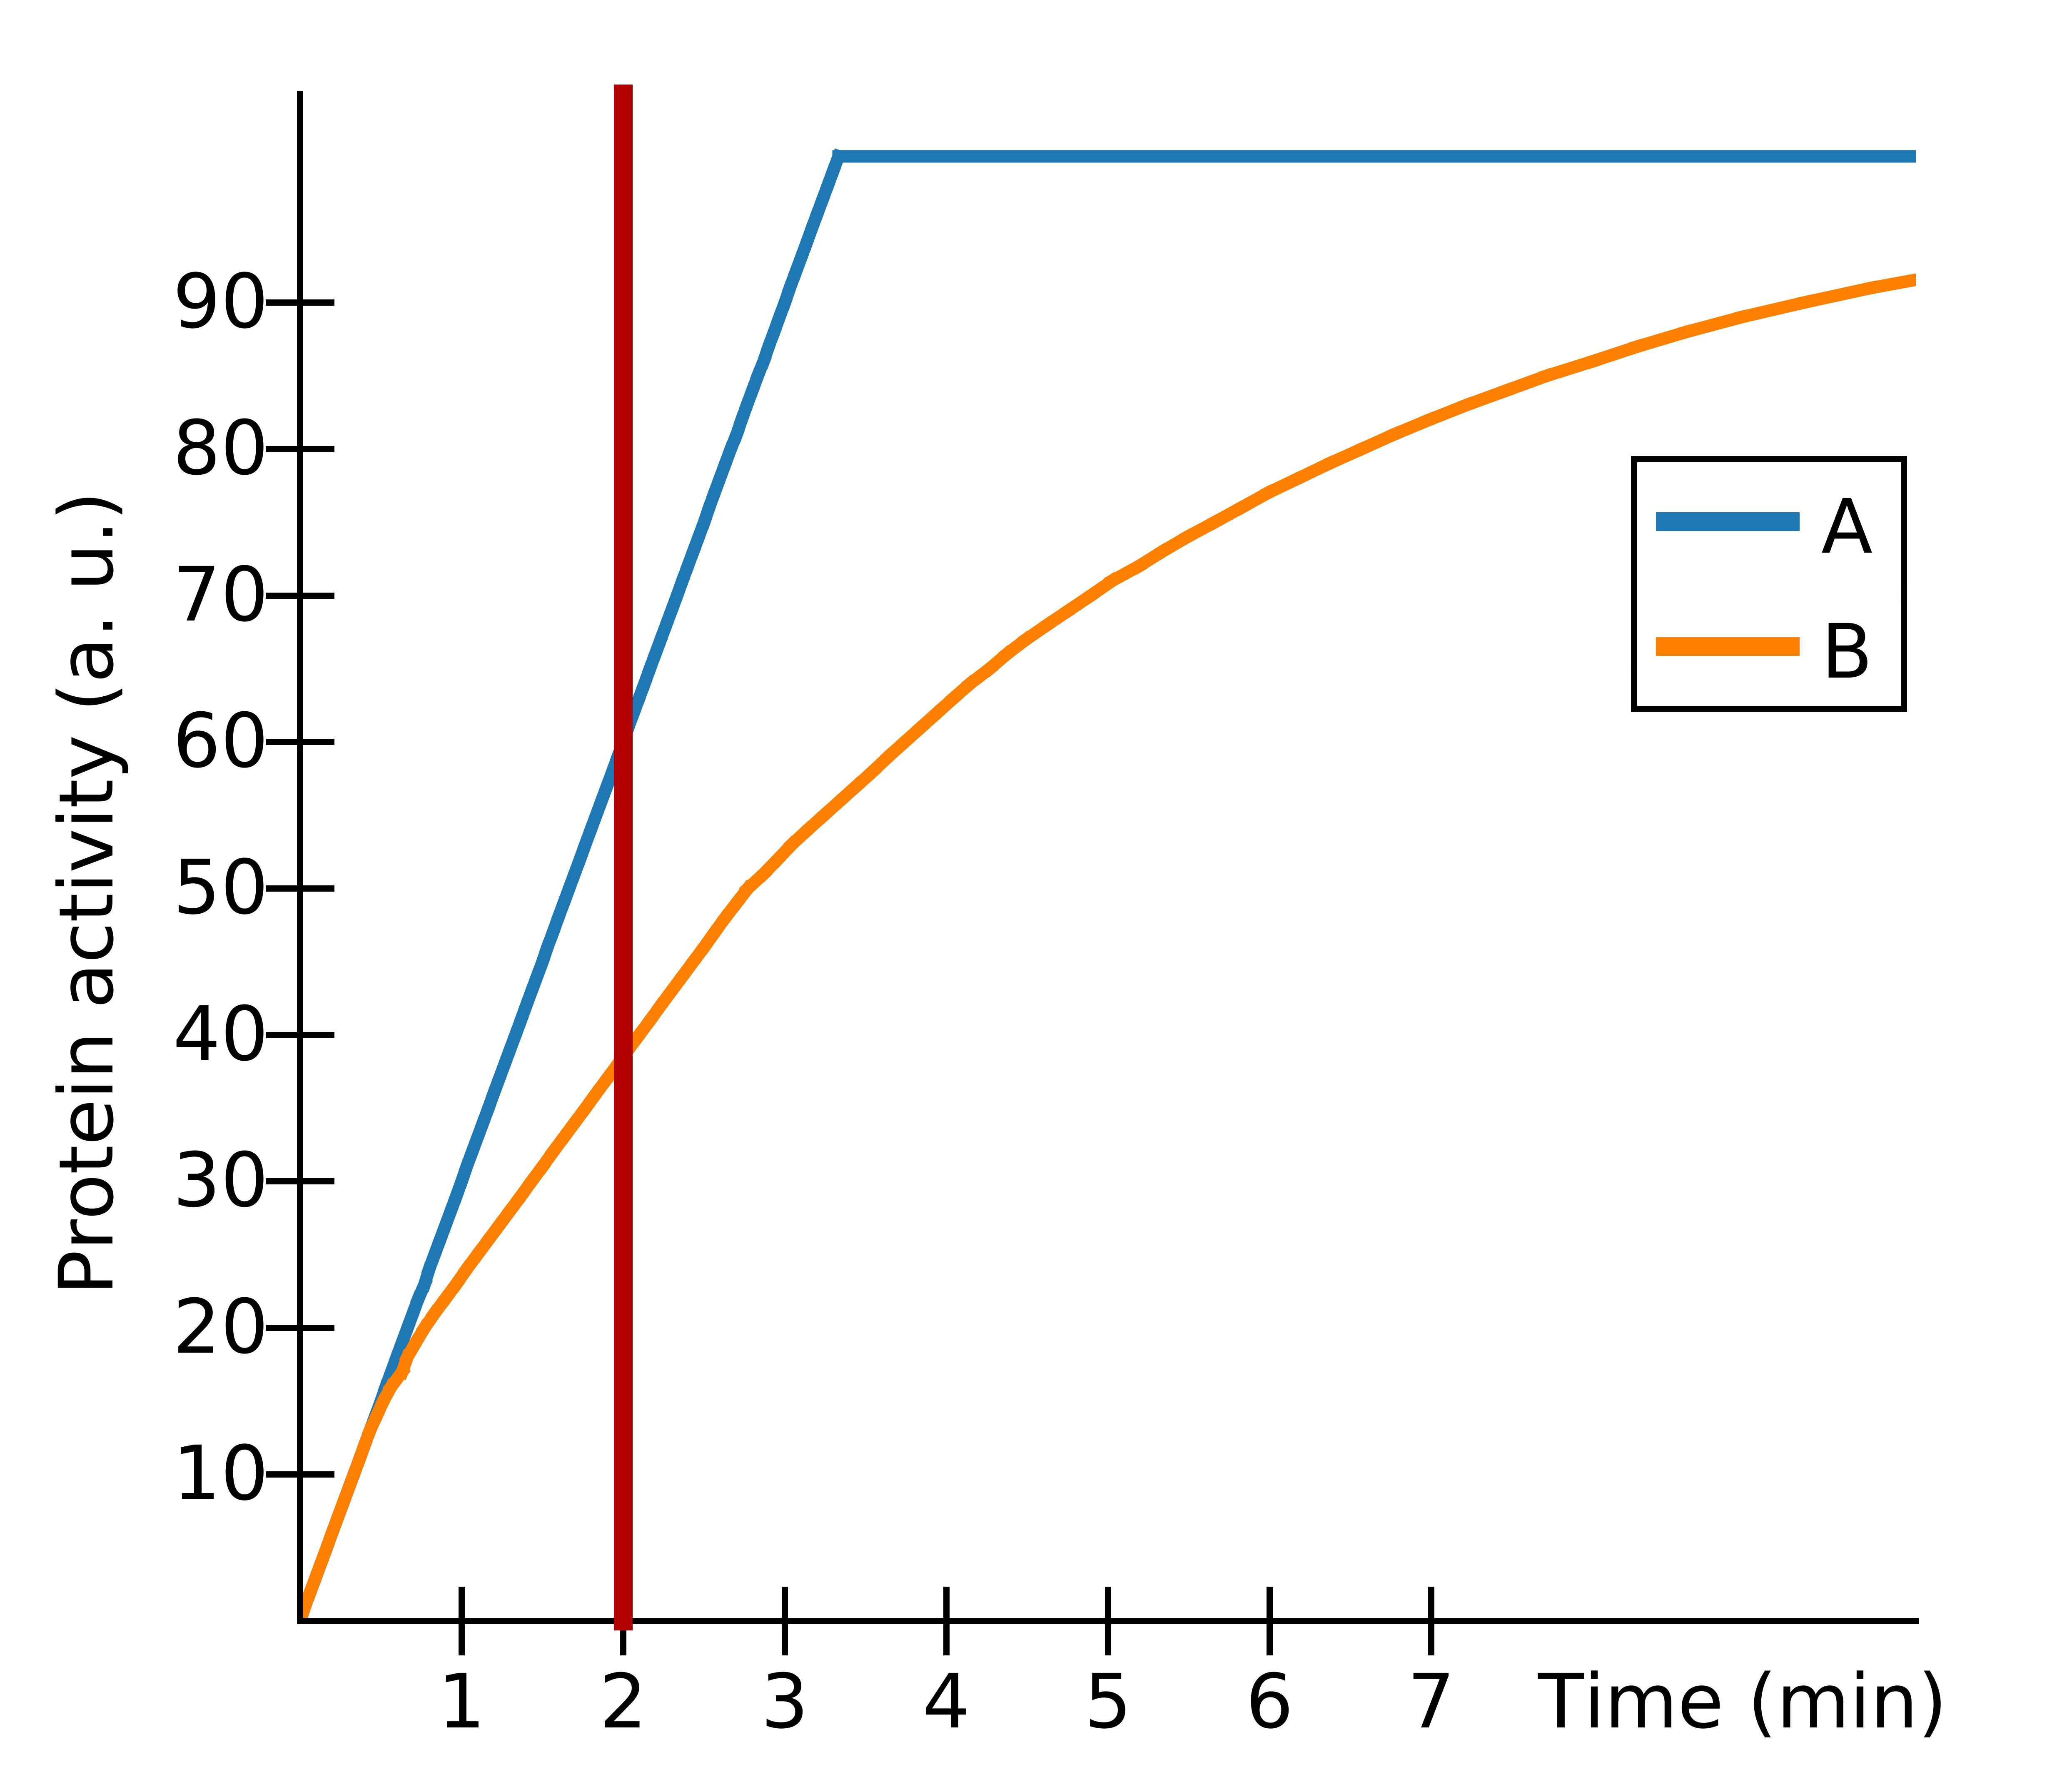
\includegraphics[scale=\graphScale]{scenario1-2_graph}} \\
\subfloat[\label{fig:animo-settings-k-network}]{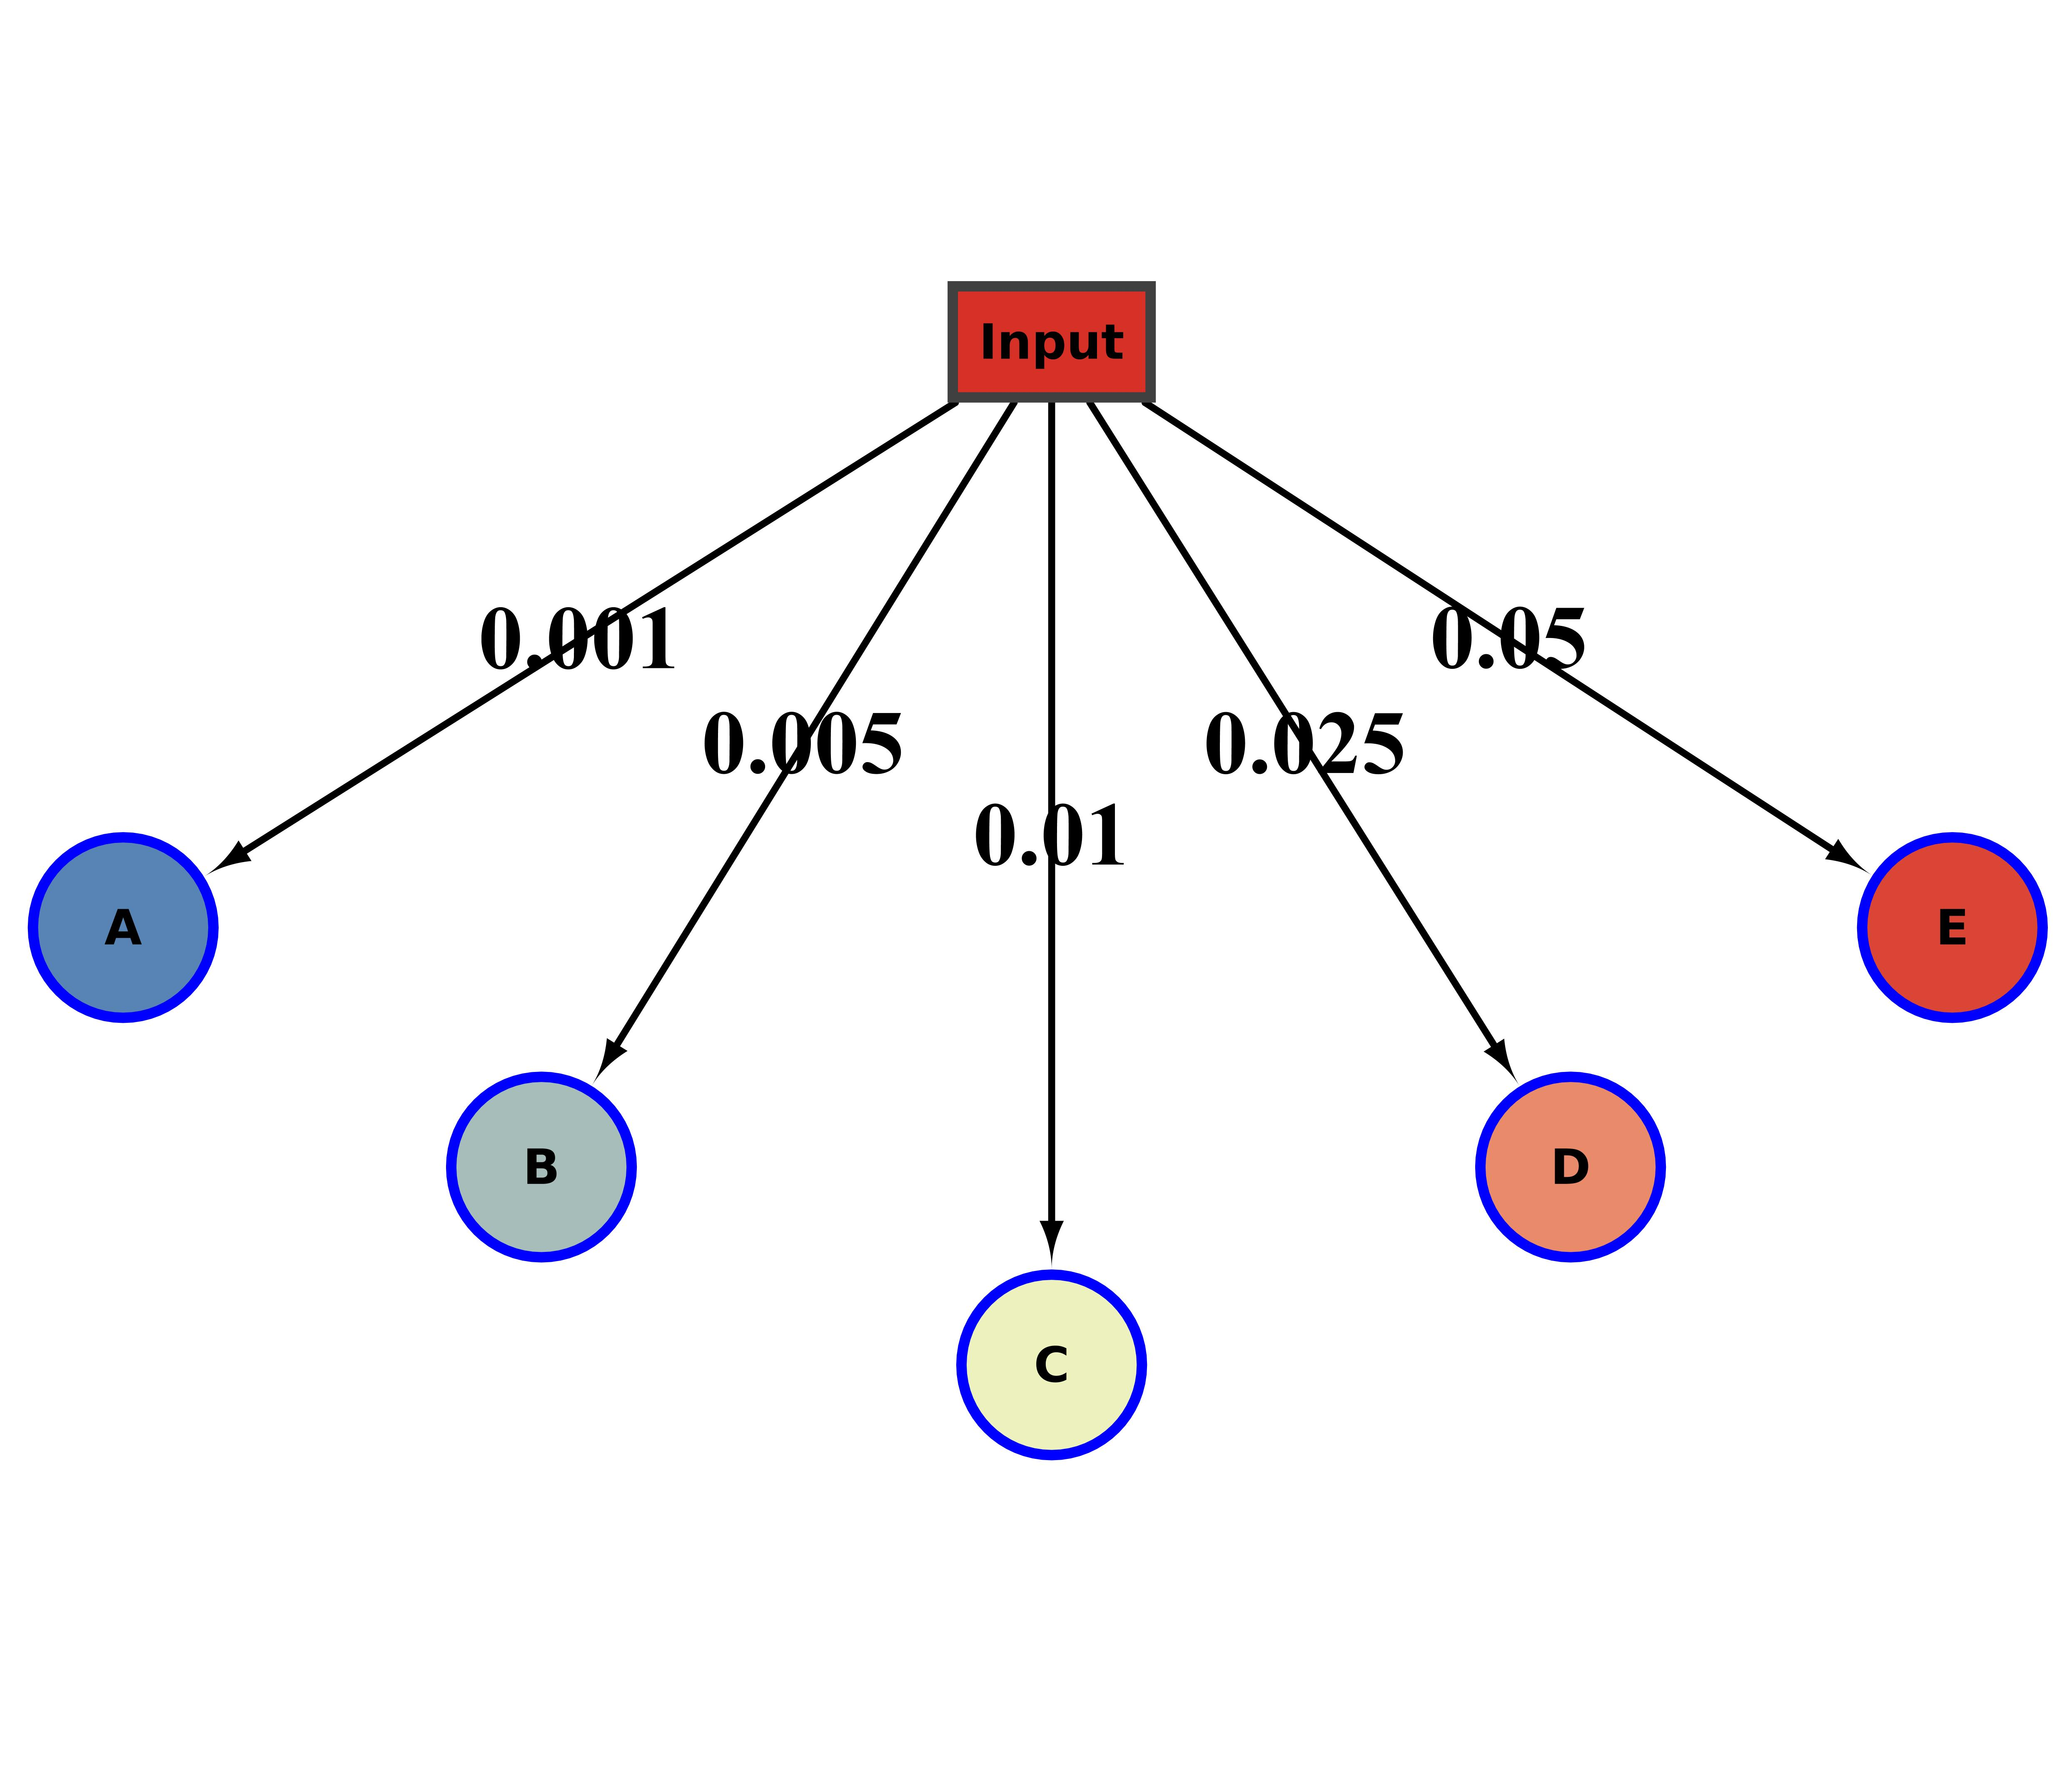
\includegraphics[scale=\graphScale]{parameter_network_CB}} &
\subfloat[\label{fig:animo-settings-k-graph}]{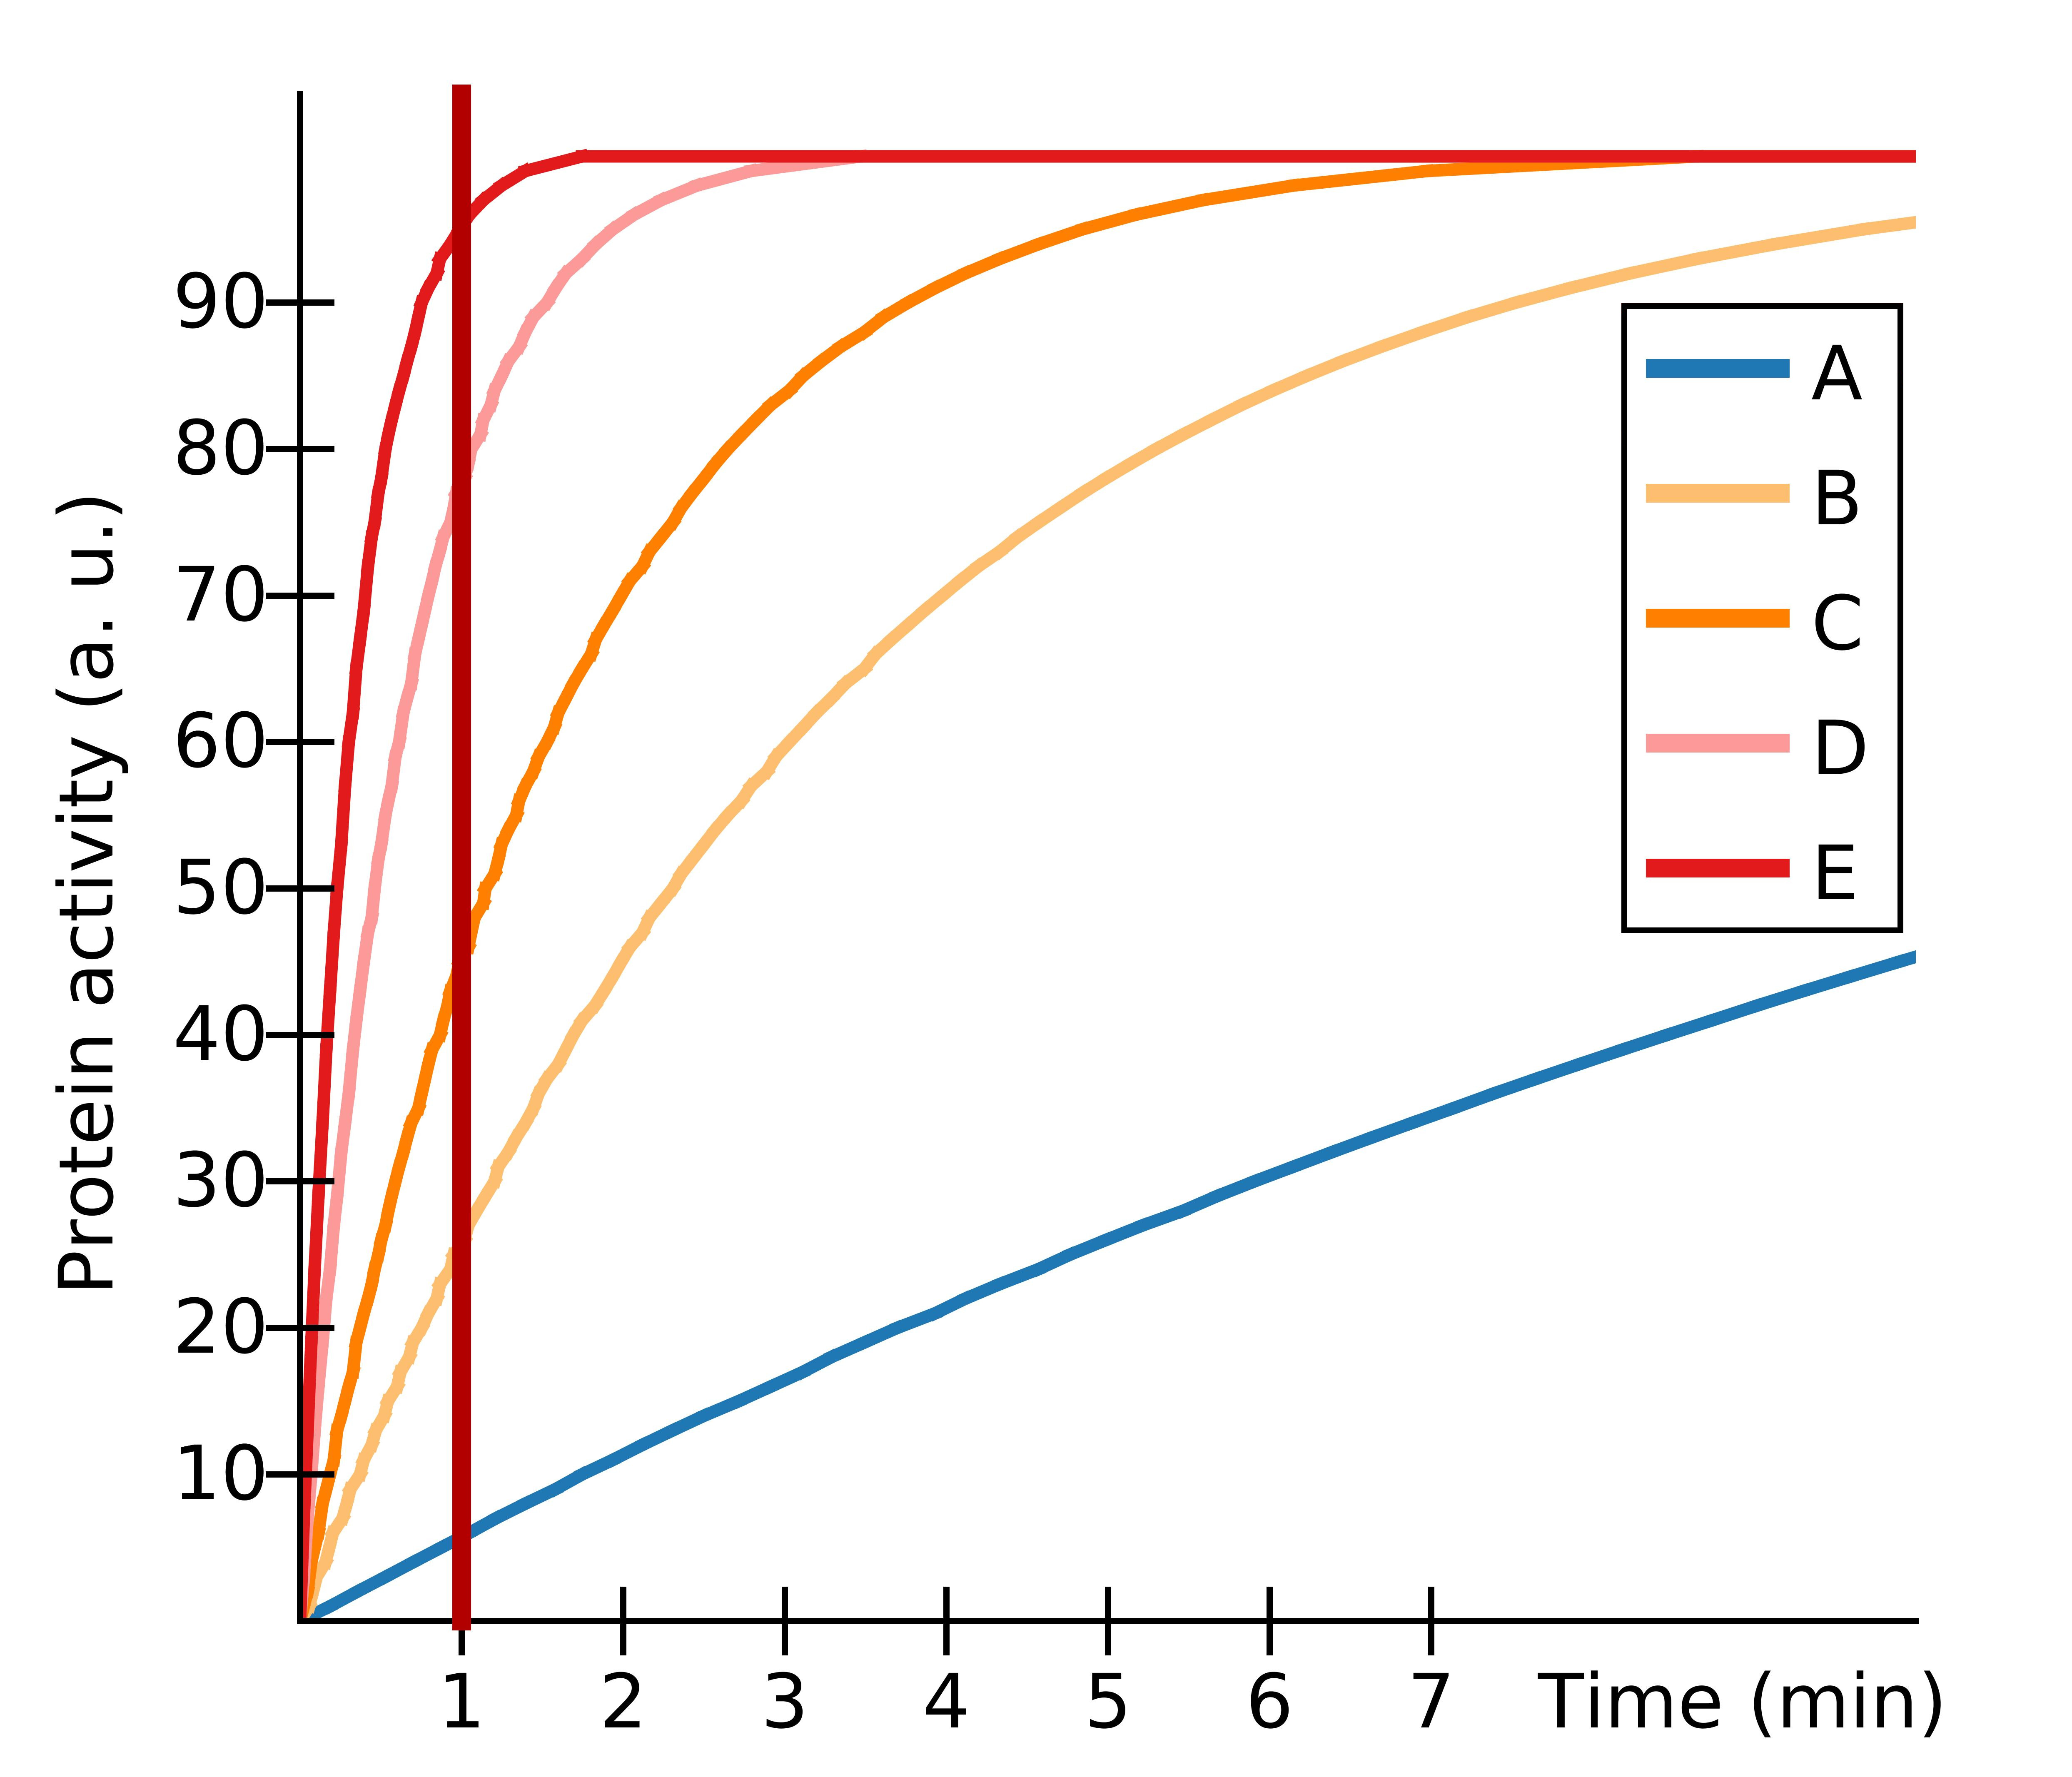
\includegraphics[scale=\graphScale]{parameter_graph}}
\end{tabular}
\caption{Example interaction settings for an ANIMO model. Each graph represents the time evolution
of the network on its left. The vertical red lines in the graphs represent the point in time on which
the coloration of the nodes in the corresponding network is based.\\
{\bf ({\protect\subref*{fig:animo-settings-scenario-network}})} The two basic scenarios. Scenario 1
makes the speed of the interaction depend only on the activity level of the upstream node {\sf Input}. In this case the
upstream node is constantly active, so the activity of {\sf A} increases linearly with time. Scenario 2
depends on the activity level of the {\sf Input} node, and on the \emph{inactivity} of {\sf B}. This
makes the rate of activation of {\sf B} decrease proportionally to the current activity level of {\sf B}:
the more {\sf B} is active, the slower the activation process will occur.\\
{\bf ({\protect\subref*{fig:animo-settings-k-network}})} Choosing a value for the scaling factor $k$. While all interactions here
are based on scenario 2, the value of their parameter $k$ (written on the edges) determines the speed at which the downstream node
is activated: a larger value of $k$ means a faster reaction.
\label{fig:animo-networks1}}
\end{figure*}


\begin{figure*}[htbp]
\centering
\begin{tabular}{ll}
\subfloat[\label{fig:animo-settings-direct-network}]{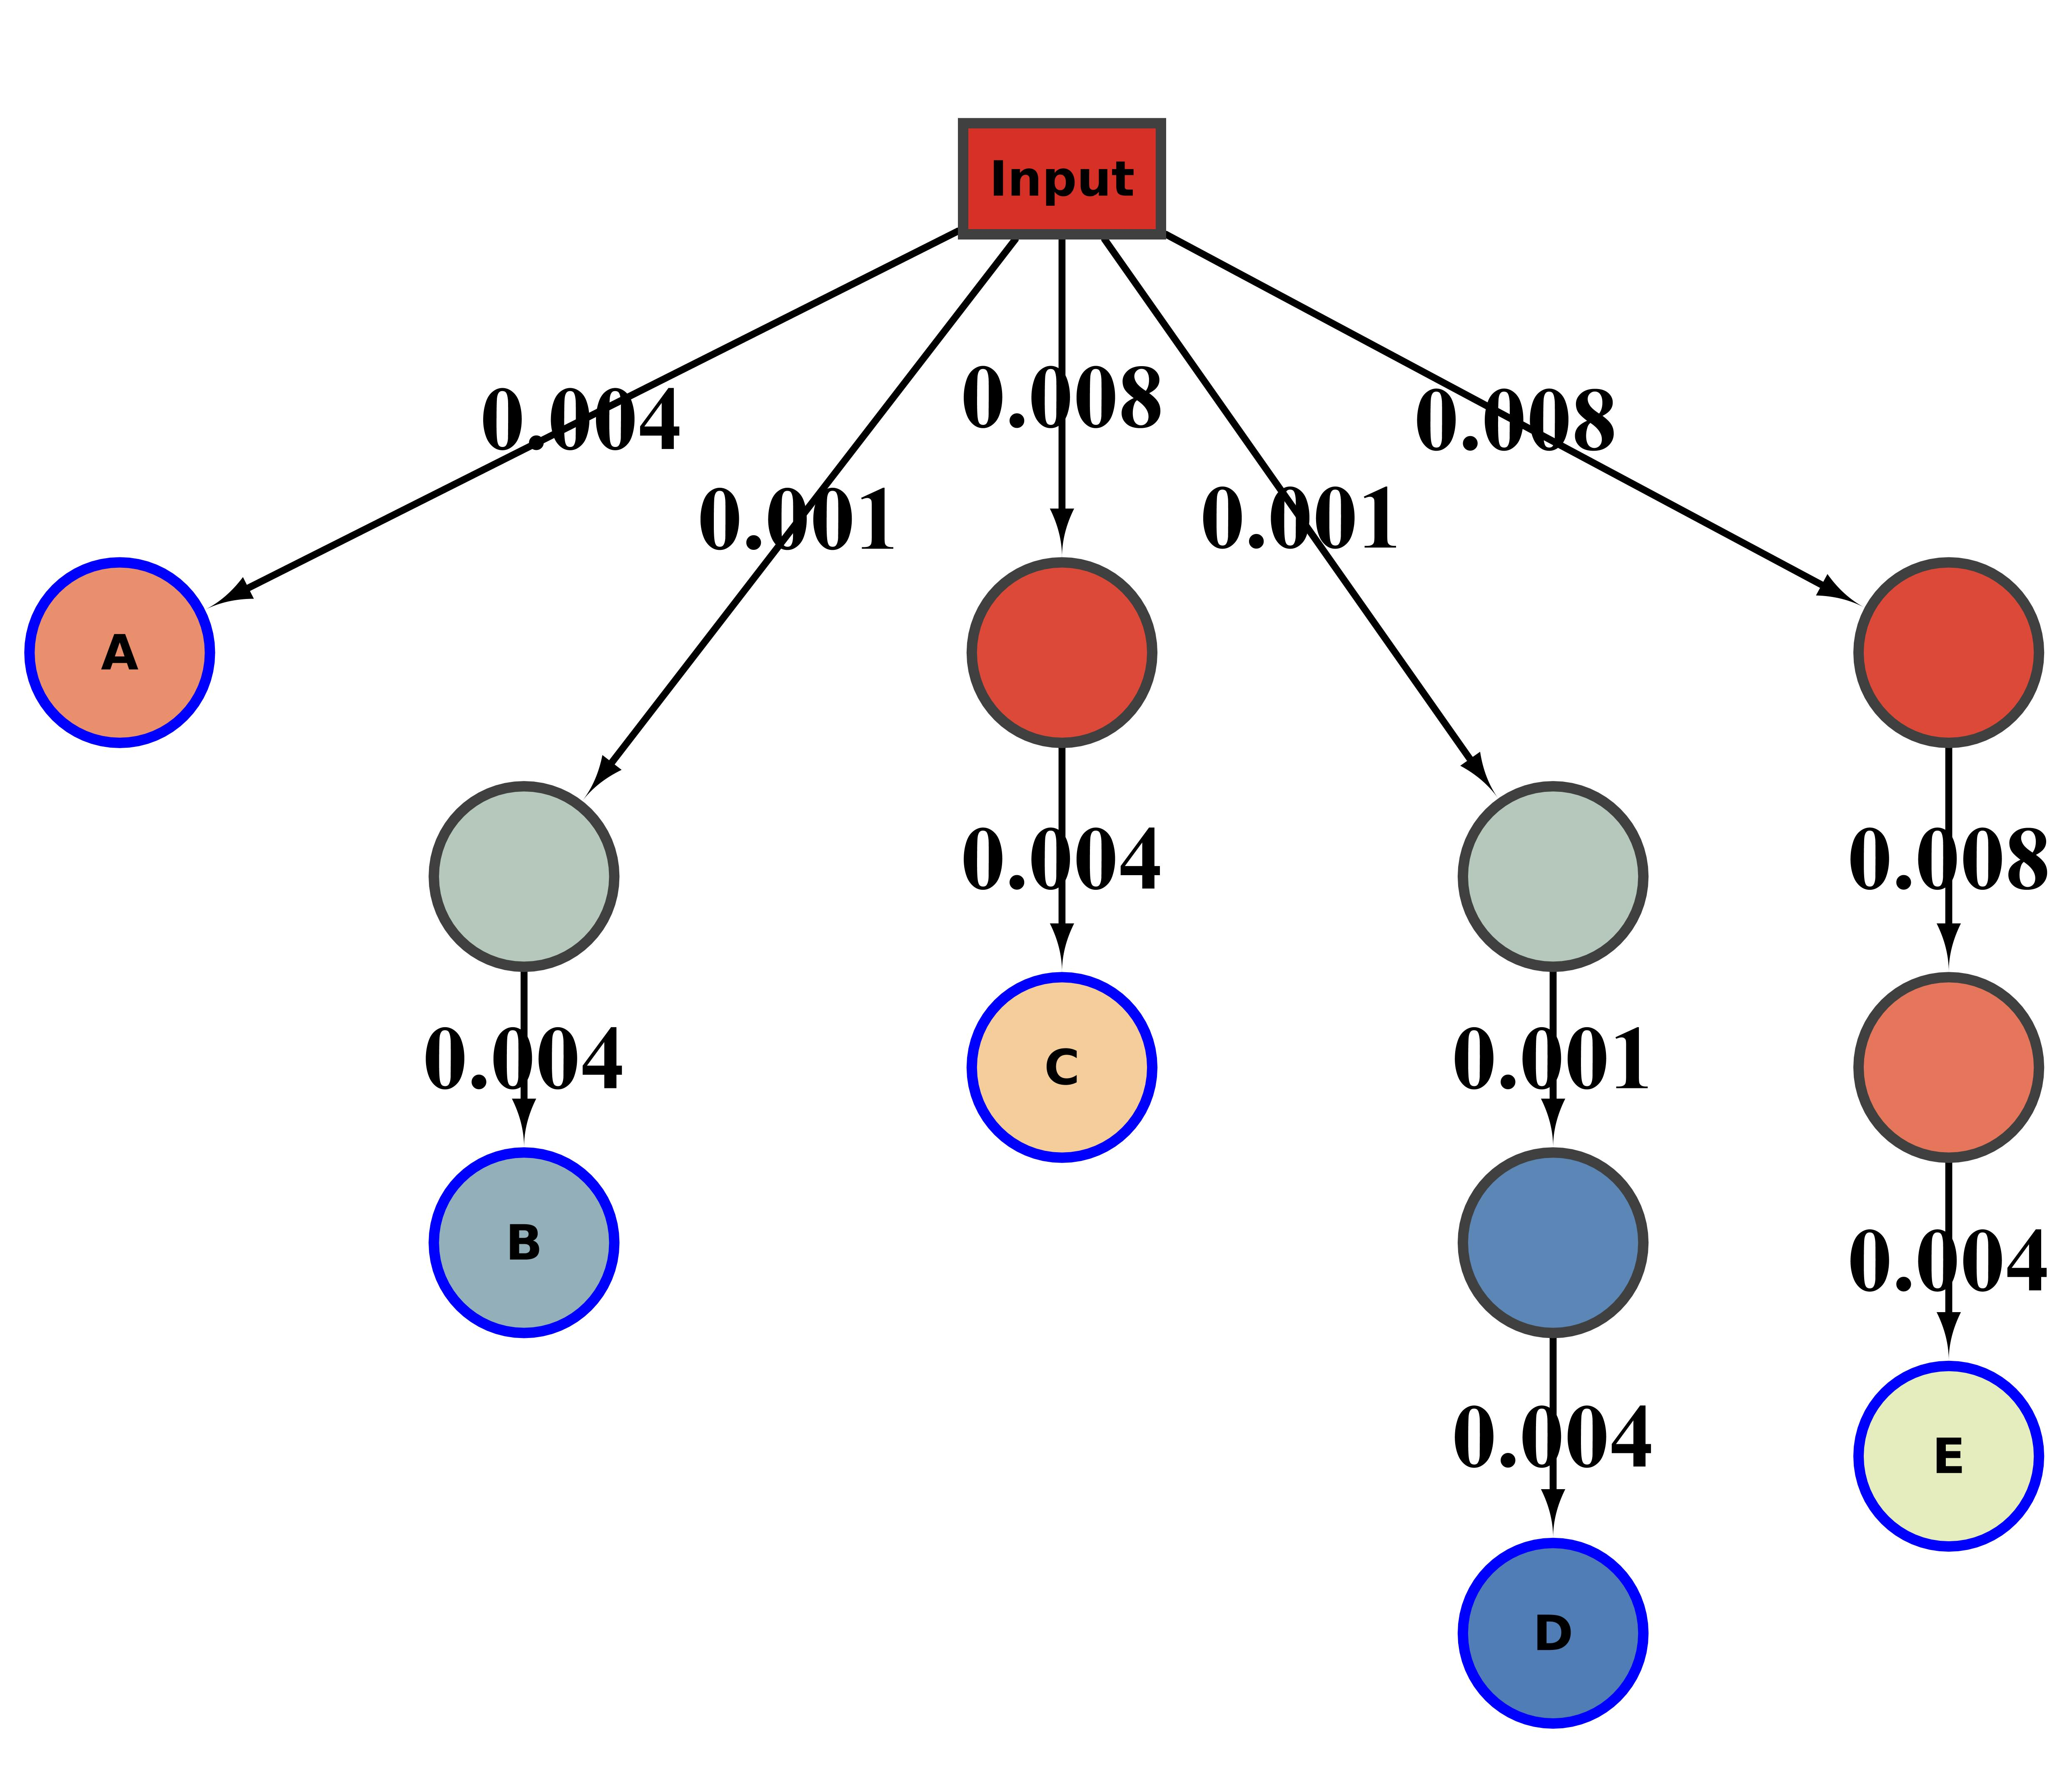
\includegraphics[scale=\graphScale]{direct_indirect_network_CB}} & 
\subfloat[\label{fig:animo-settings-direct-graph}]{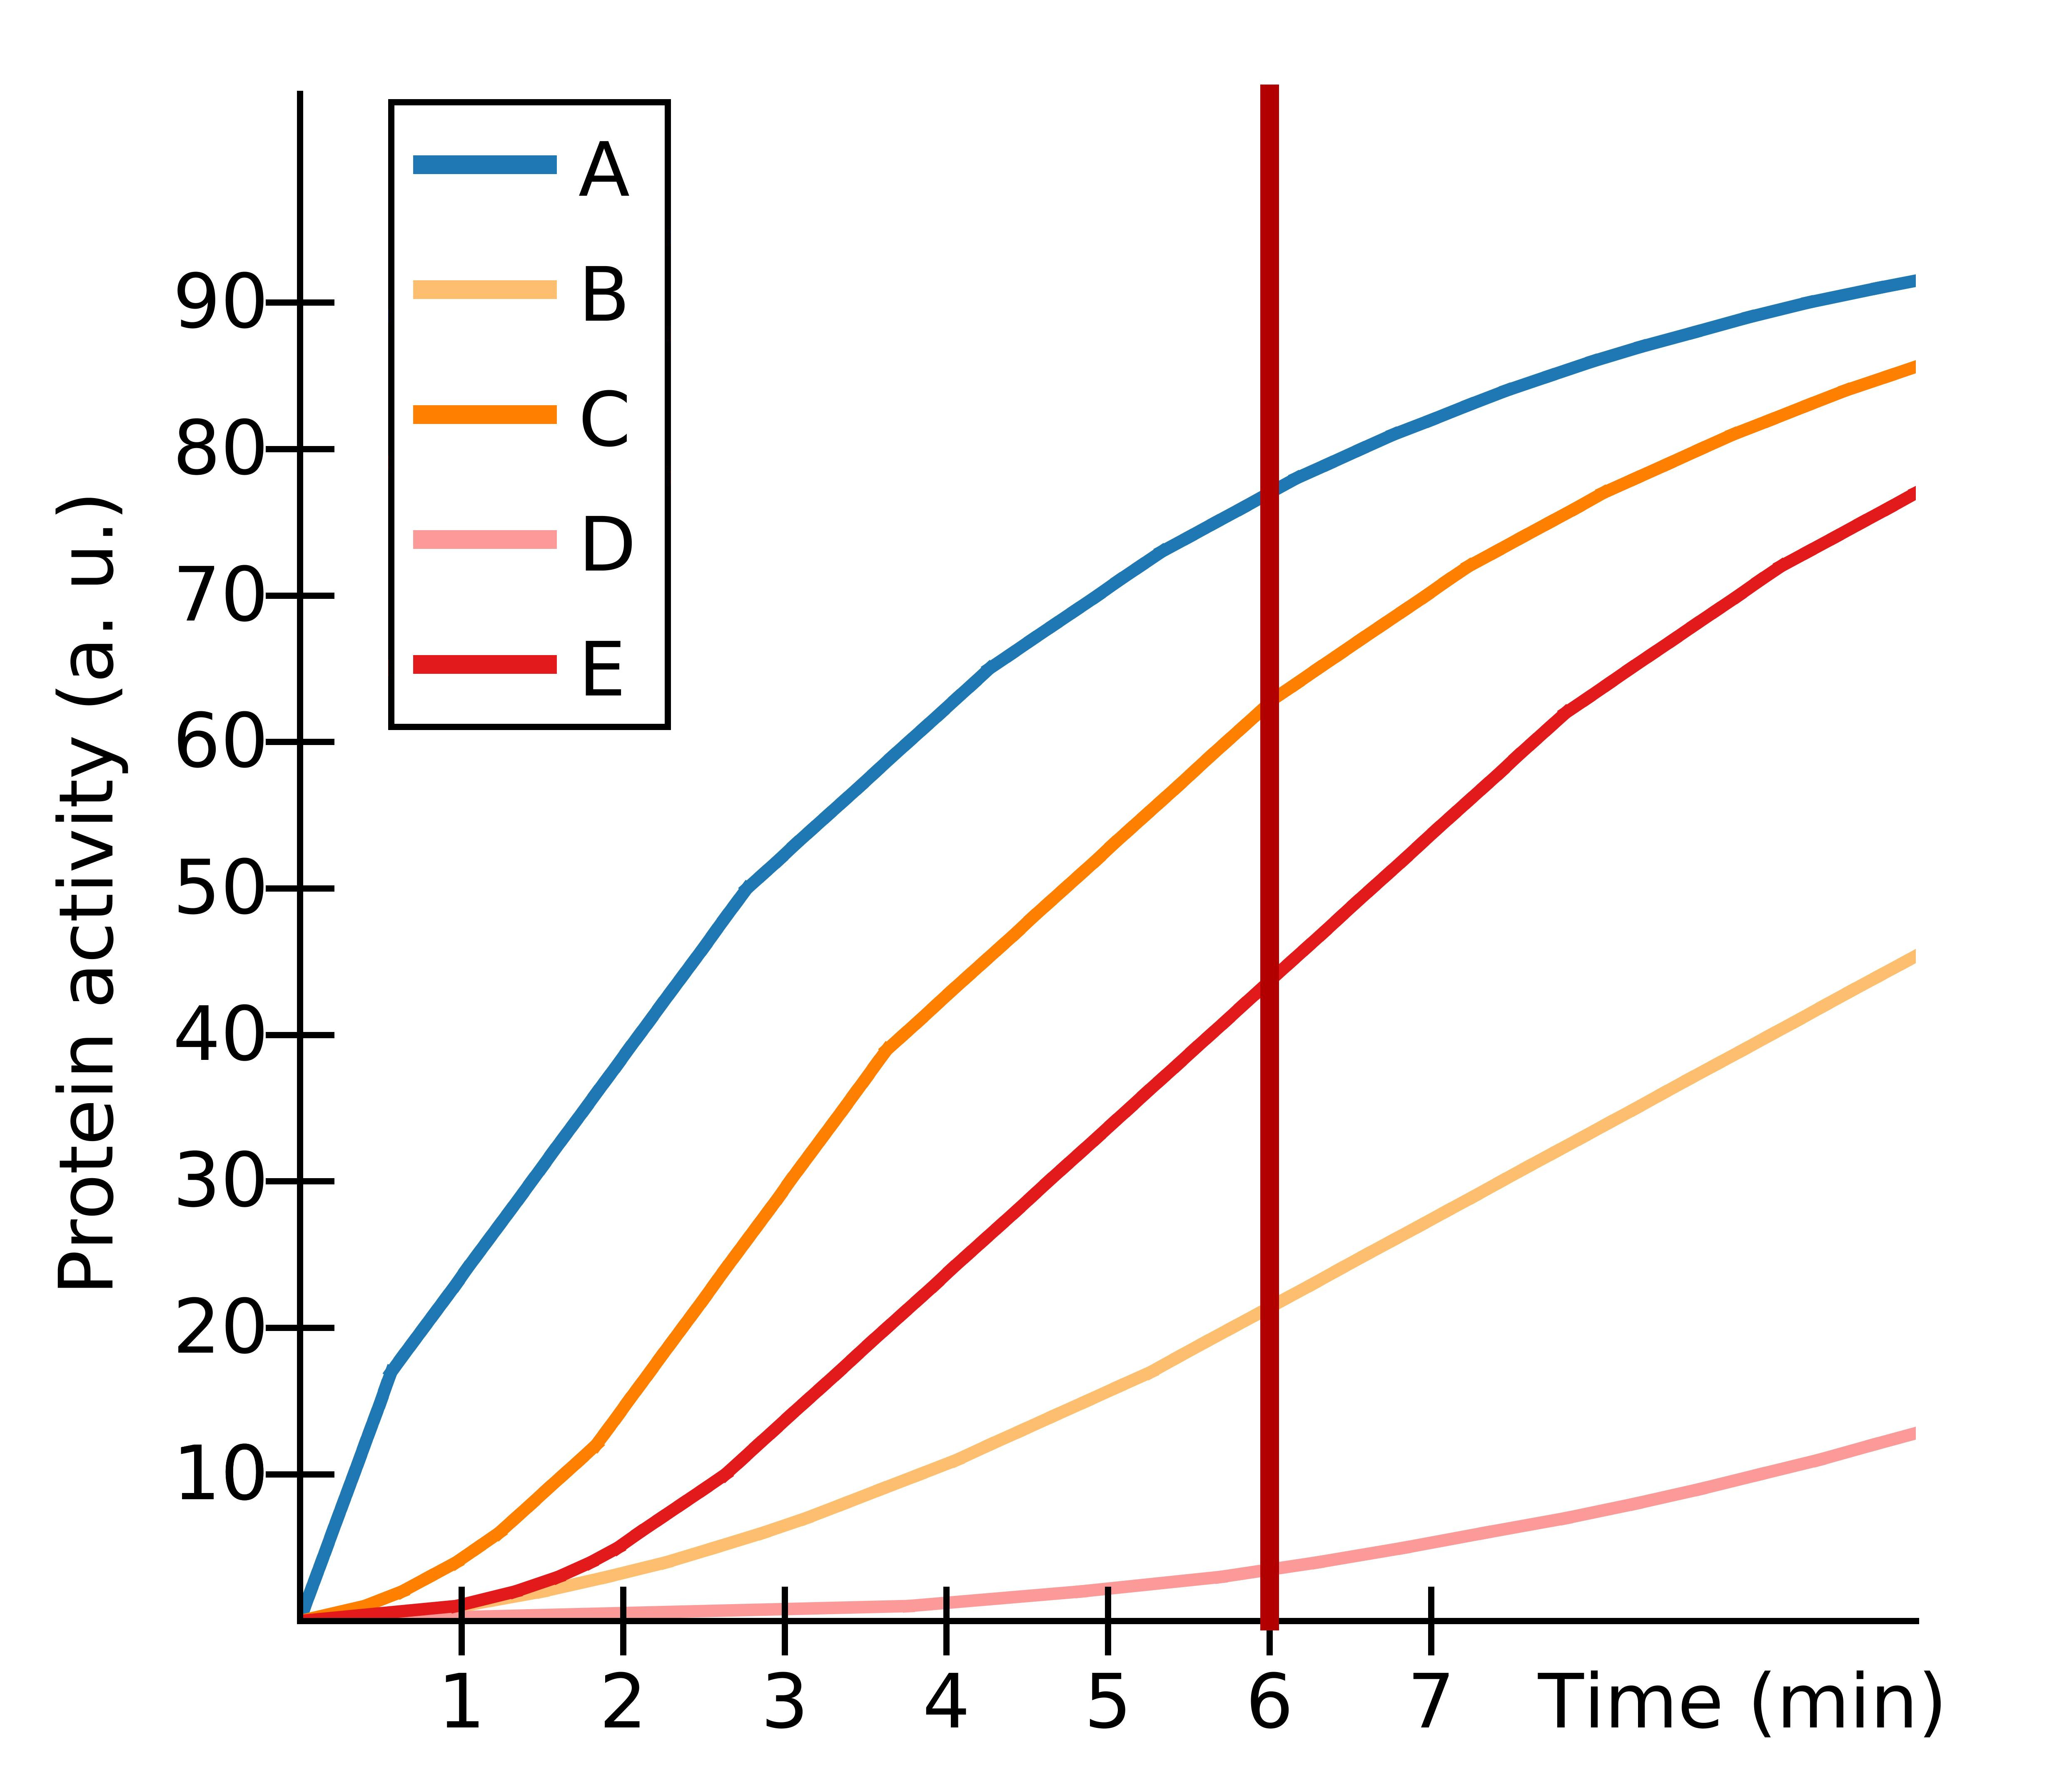
\includegraphics[scale=\graphScale]{direct_indirect_graph}} \\ 
\subfloat[\label{fig:animo-settings-feedback-network}]{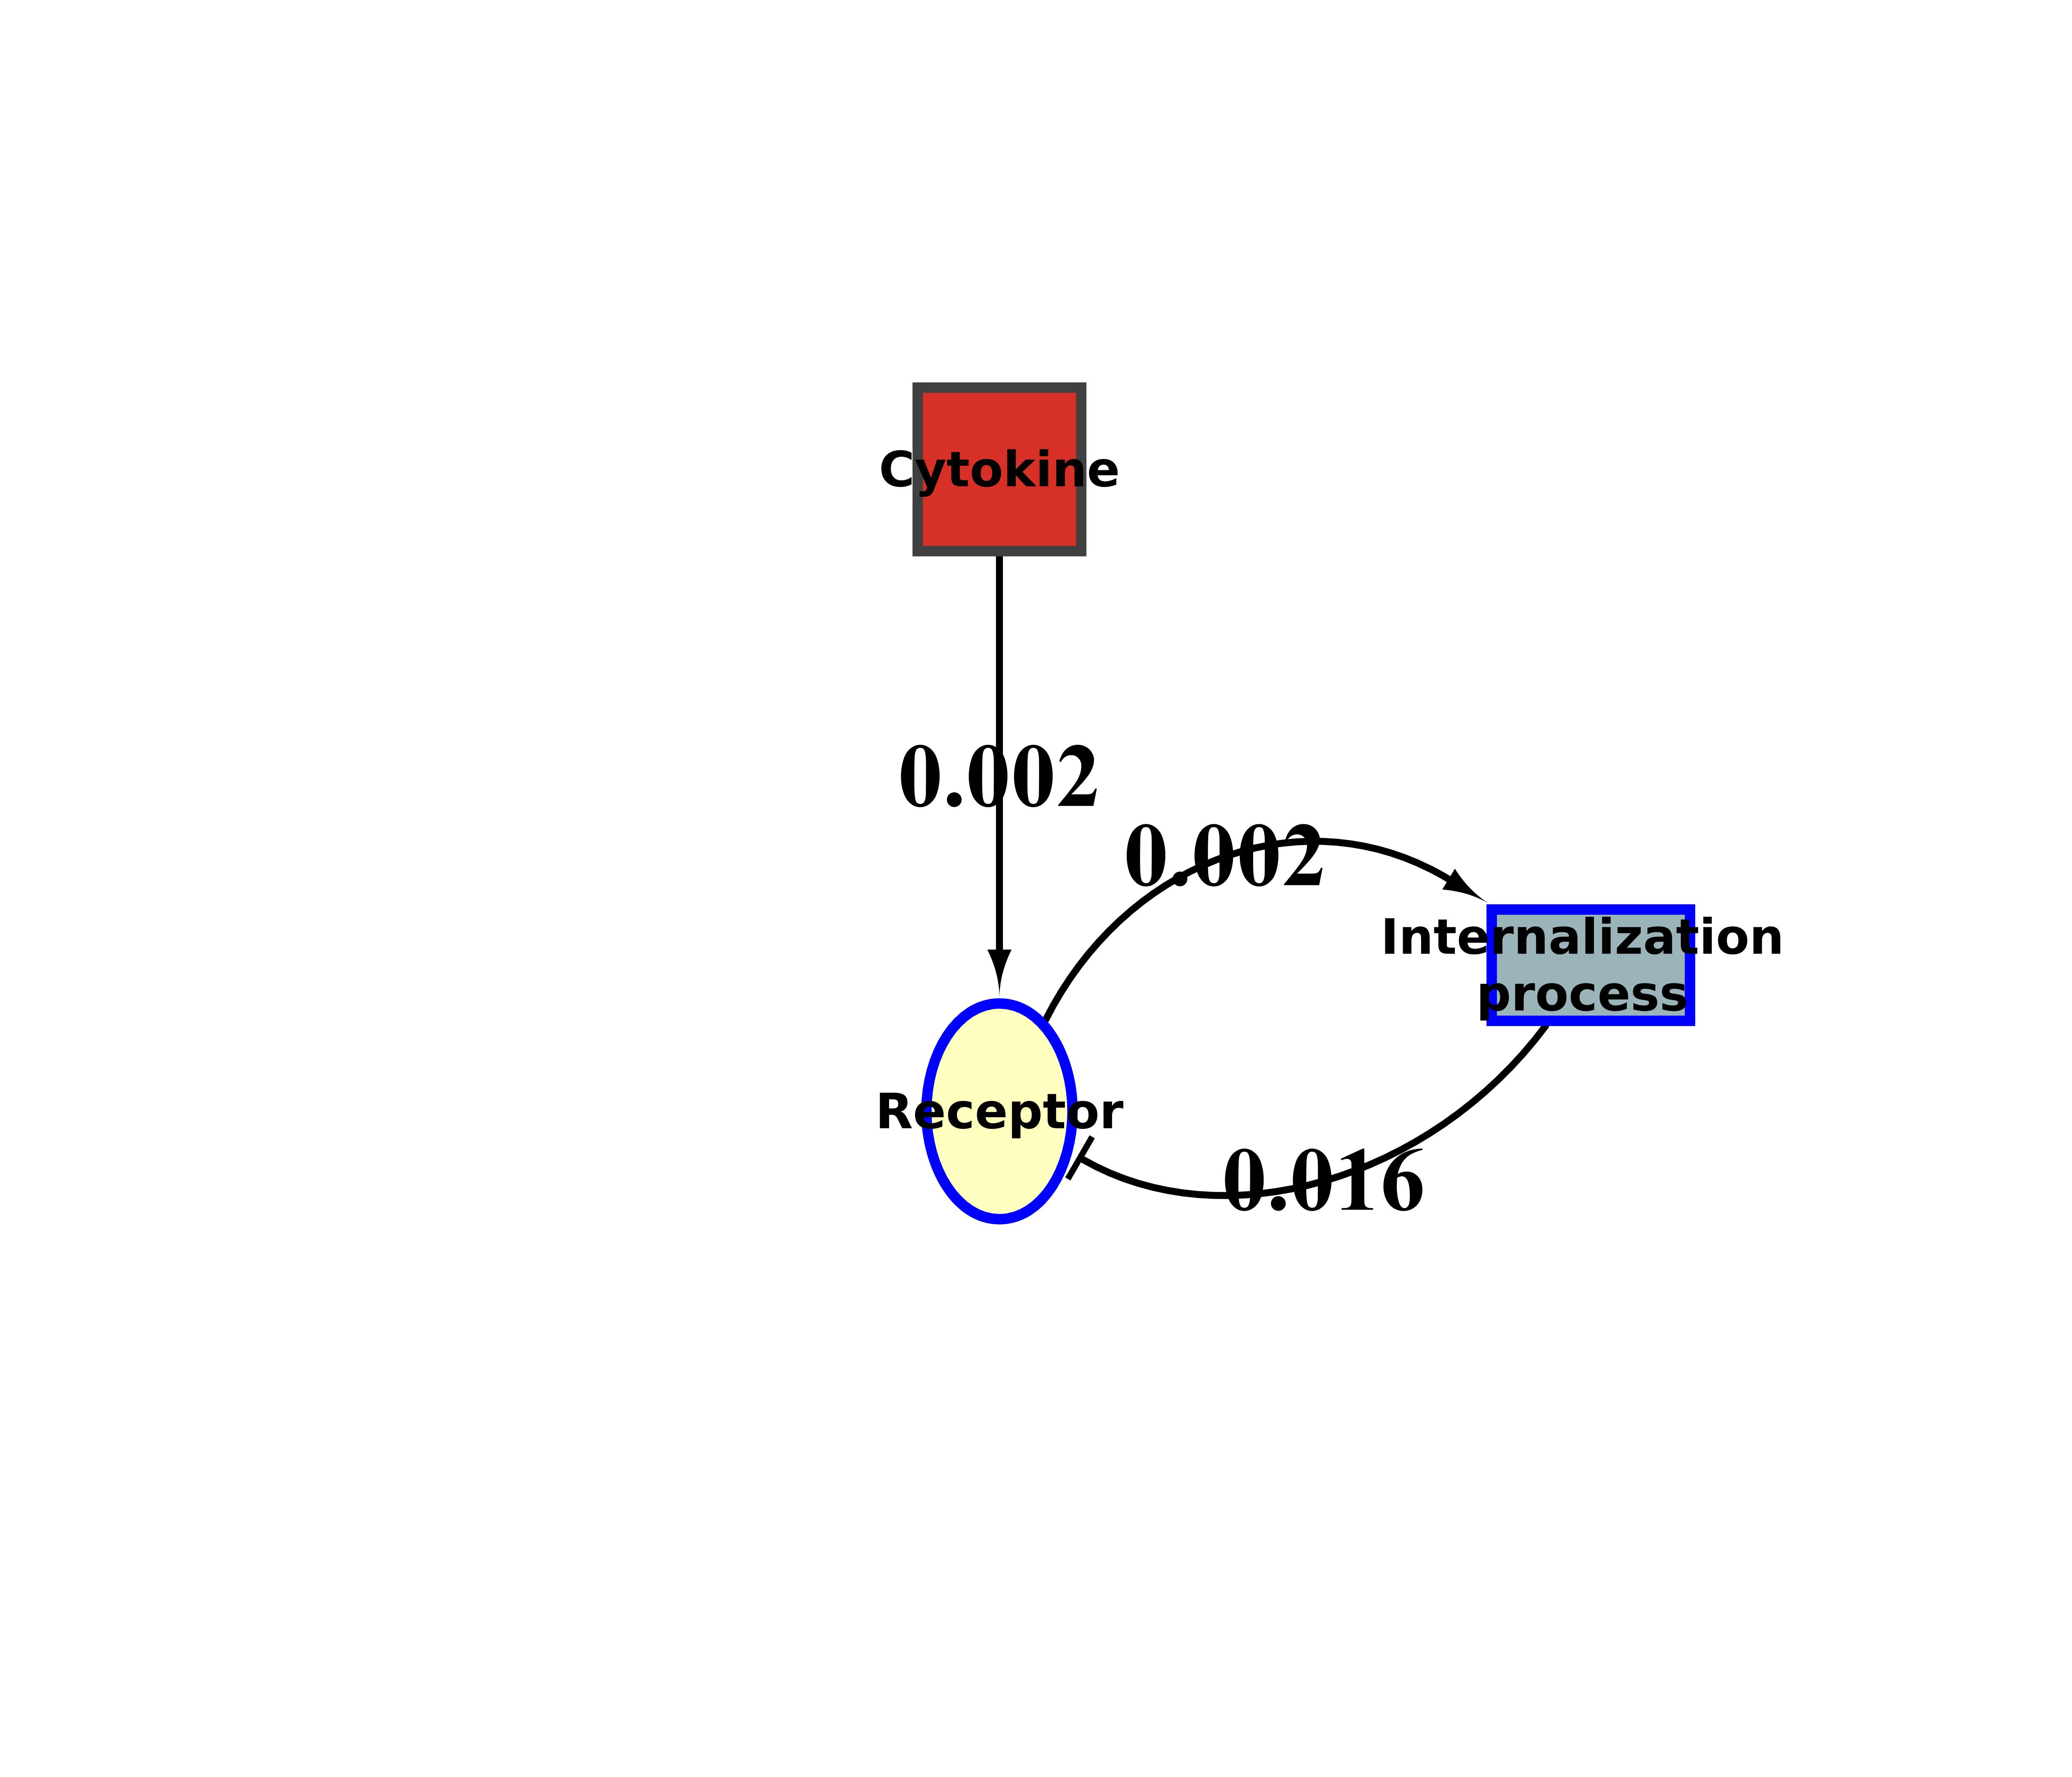
\includegraphics[scale=\graphScale]{feedback_network_CB}} & 
\subfloat[\label{fig:animo-settings-feedback-graph}]{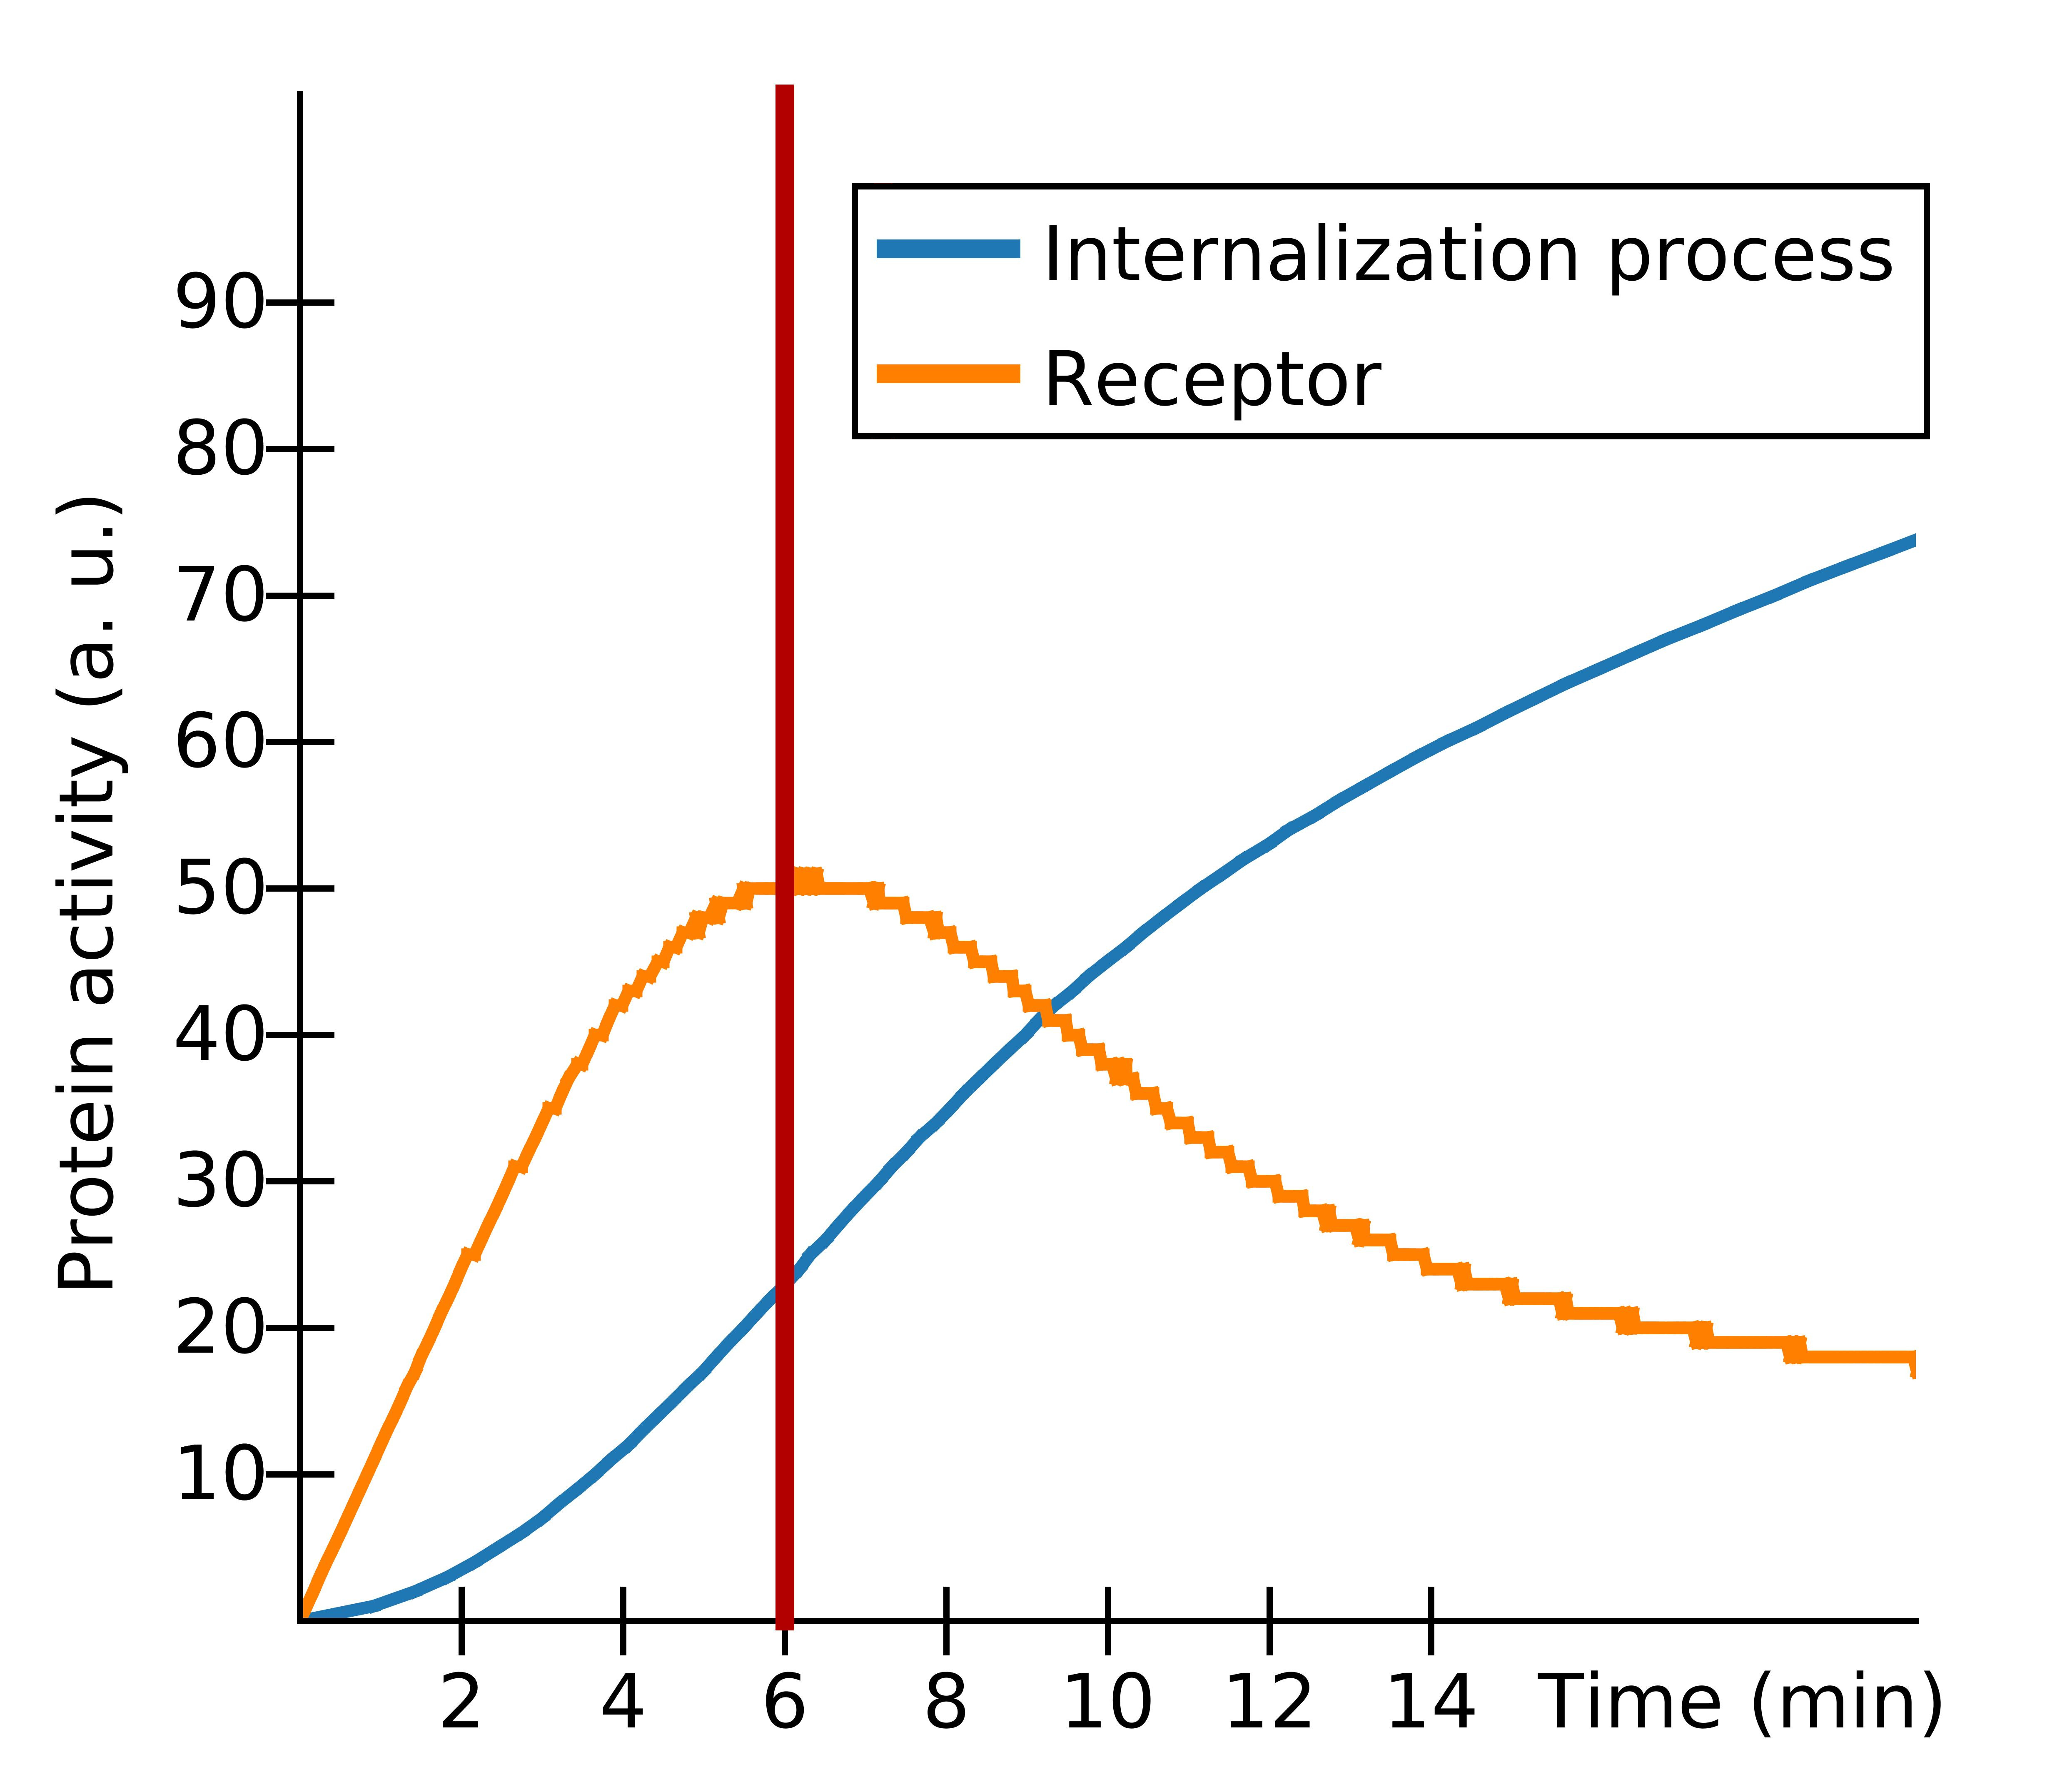
\includegraphics[scale=\graphScale]{feedback_graph}}
\end{tabular}
\caption{Example interaction settings for an ANIMO model. Each graph represents the time evolution
of the network on its left. The vertical red lines in the graphs represent the point in time on which
the coloration of the nodes in the corresponding network is based.\\
{\bf ({\protect\subref*{fig:animo-settings-direct-network}})} Relation between network topology and delays. In order to delay the activation process
ensuing an external signal (node {\sf Input}), we can reduce the reaction speed by changing $k$ or
adding an intermediate node. Introducing a slowly activated ($k = 0.001$) node between {\sf Input} and {\sf B} is enough to
activate {\sf B} at a much slower rate than {\sf A}, even if the value of $k$ for the last step is left unchanged at $k = 0.004$.
Increasing the parameter of the newly introduced reaction lets us fine tune
the speed of the response, making the activation of {\sf C} faster than {\sf B}, but still slower than {\sf A}. We repeat the process
of introducing a delay with nodes {\sf D} and {\sf E}: an additional intermediate node further reduces the response time.\\
{\bf ({\protect\subref*{fig:animo-settings-feedback-network}})} Peak dynamics are often observed in experimental data.
In order to have the activity level of a node increase and successively decrease, the simplest way is to model it with a feed-back loop.
In the example, we model the internalization of a receptor following its activation. Note that the interaction {\sf Internalization
process} $\dashv$ {\sf Receptor} is an inhibition: being based on scenario 2, it will reduce the activity of the {\sf Receptor} node with a rate proportional
to the current activity of both involved nodes. Scenario 1 dynamics are sufficient to model the two activating reactions {\sf Cytokine} $\rightarrow$ {\sf Receptor}
and {\sf Receptor} $\rightarrow$ {\sf Internalization Process}. Key to the peak dynamics is the fact that the inactivation of the {\sf Receptor} node
is much faster (higher $k$ value) than its activation.
\label{fig:animo-networks2}}
\end{figure*}

%Full figure in one page:
% \def\graphScale{0.0243}
% \begin{figure*}[htbp]
% \centering
% \begin{tabular}{llll}
% \subfloat[\label{fig:animo-settings-scenario-network}]{\includegraphics[scale=\graphScale]{scenario1-2_network_legend_CB}} &
% \subfloat[\label{fig:animo-settings-scenario-graph}]{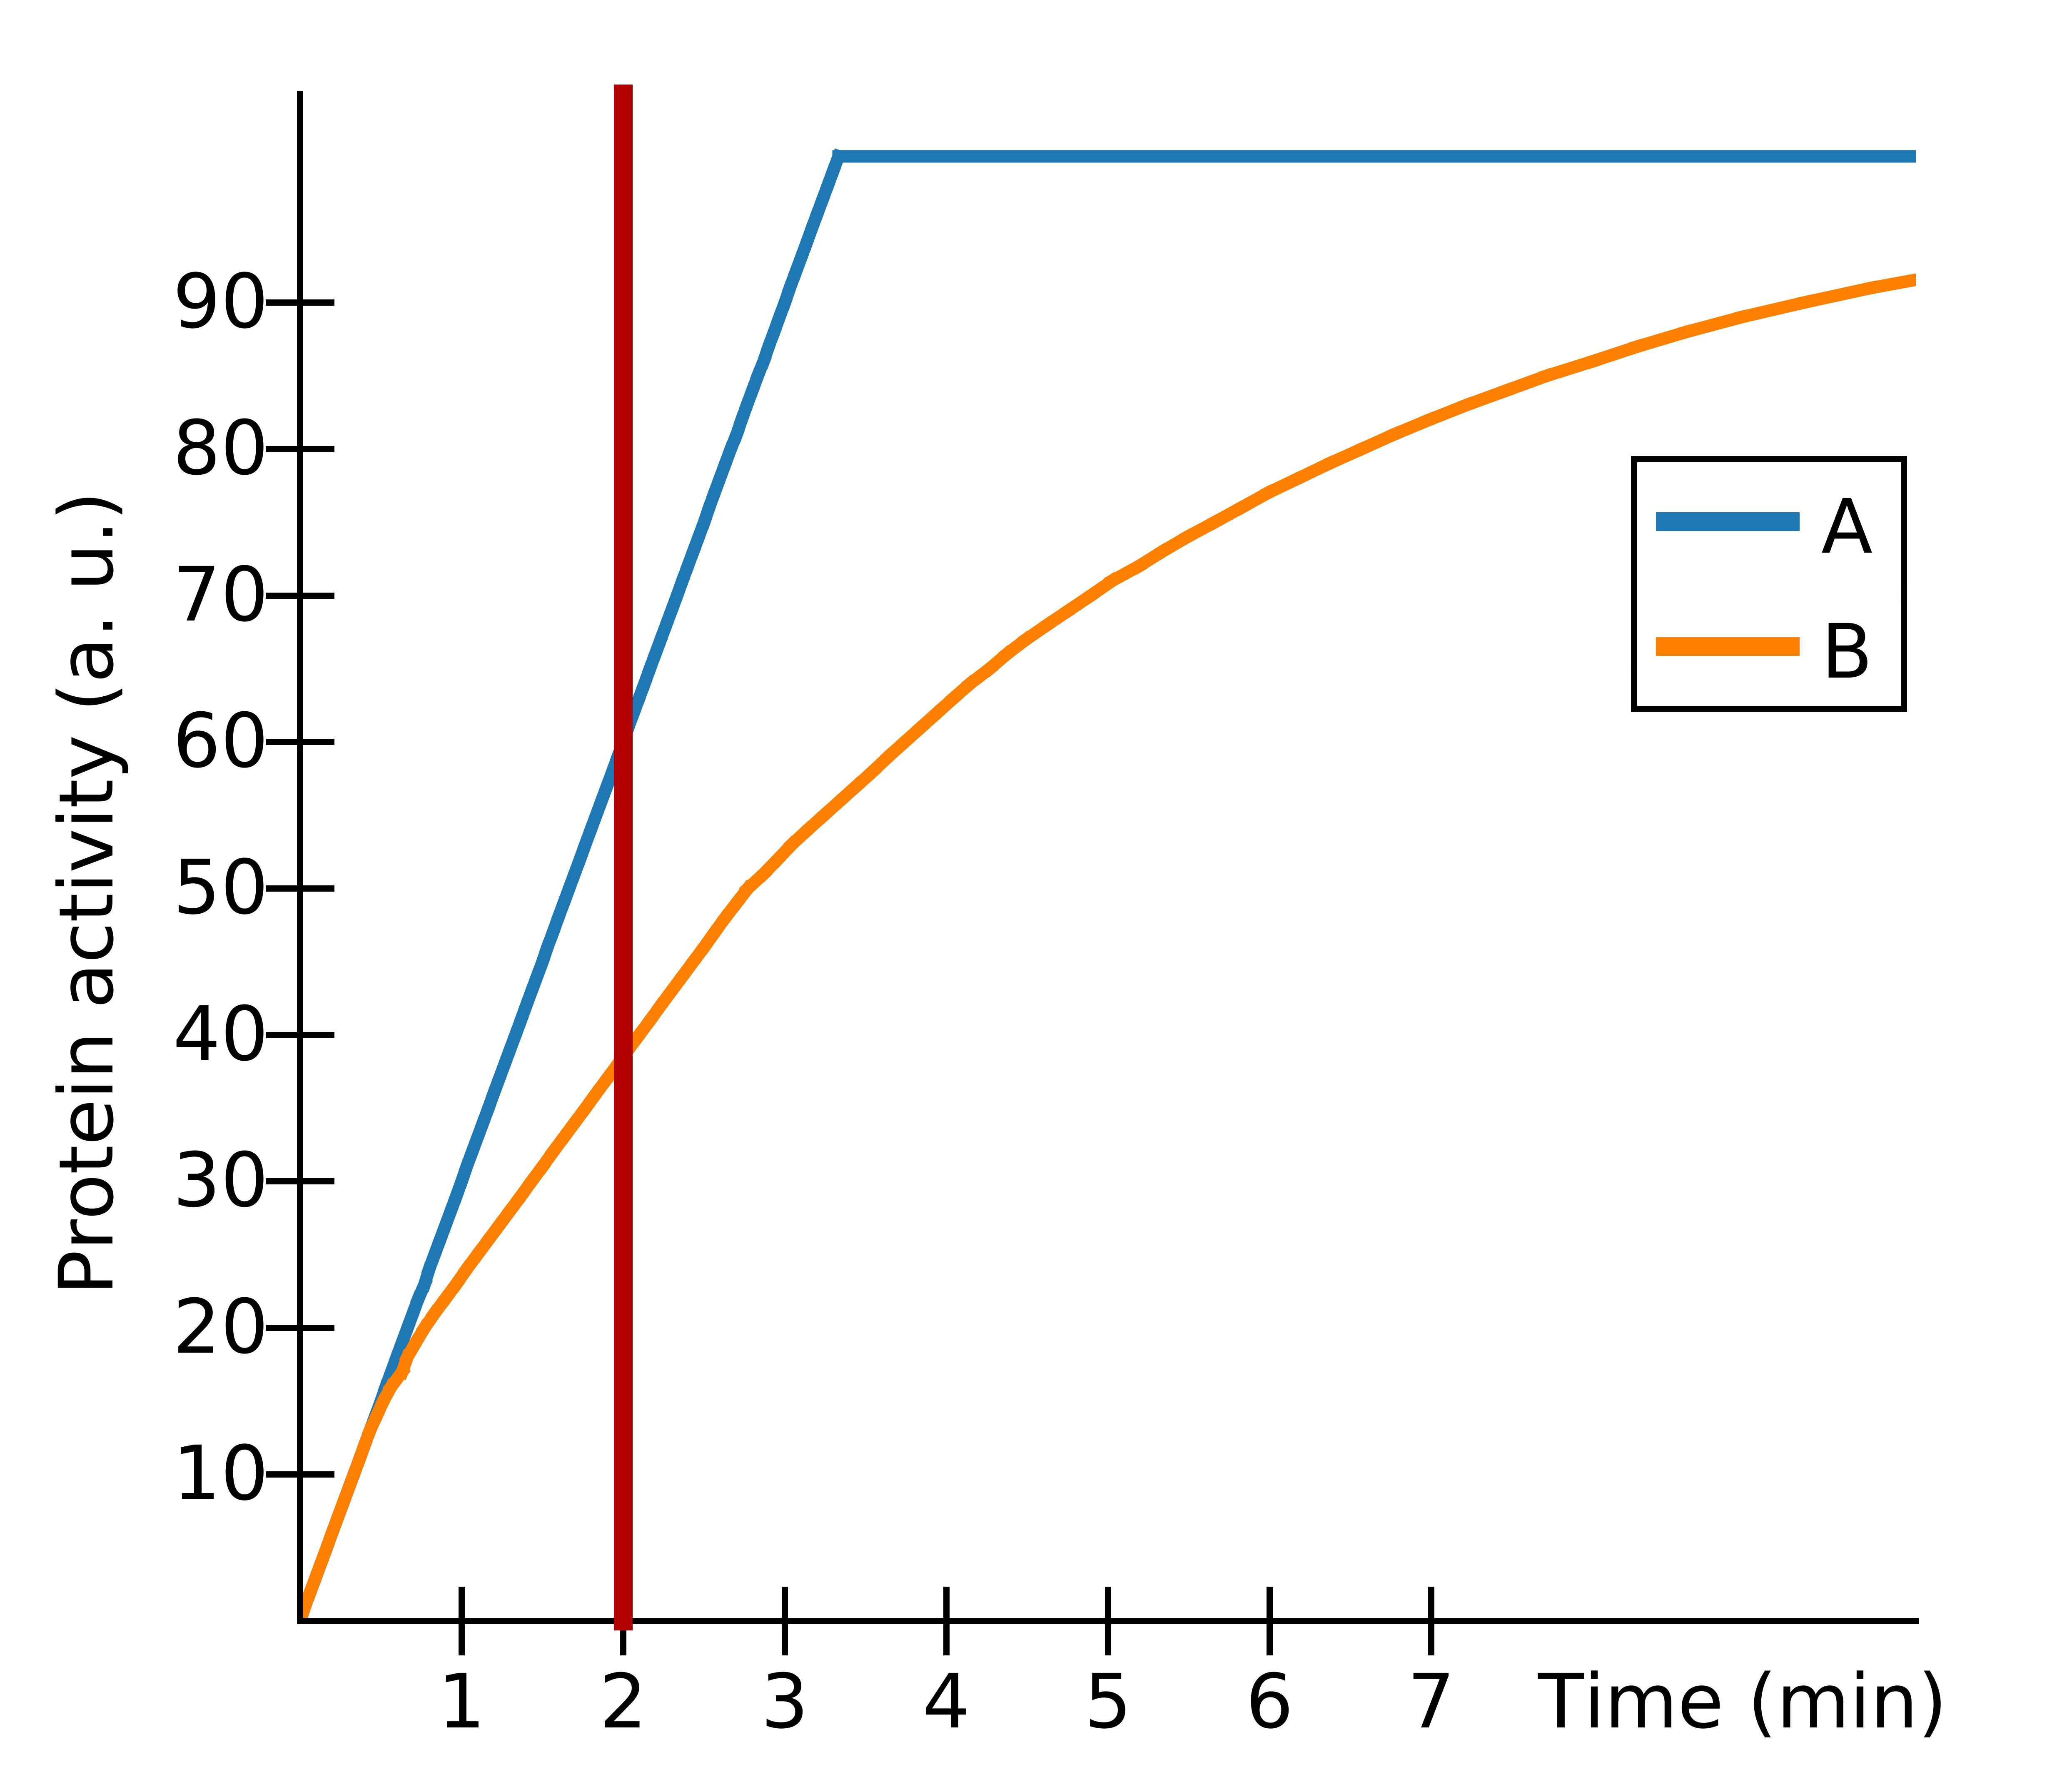
\includegraphics[scale=\graphScale]{scenario1-2_graph}} &
% \subfloat[\label{fig:animo-settings-k-network}]{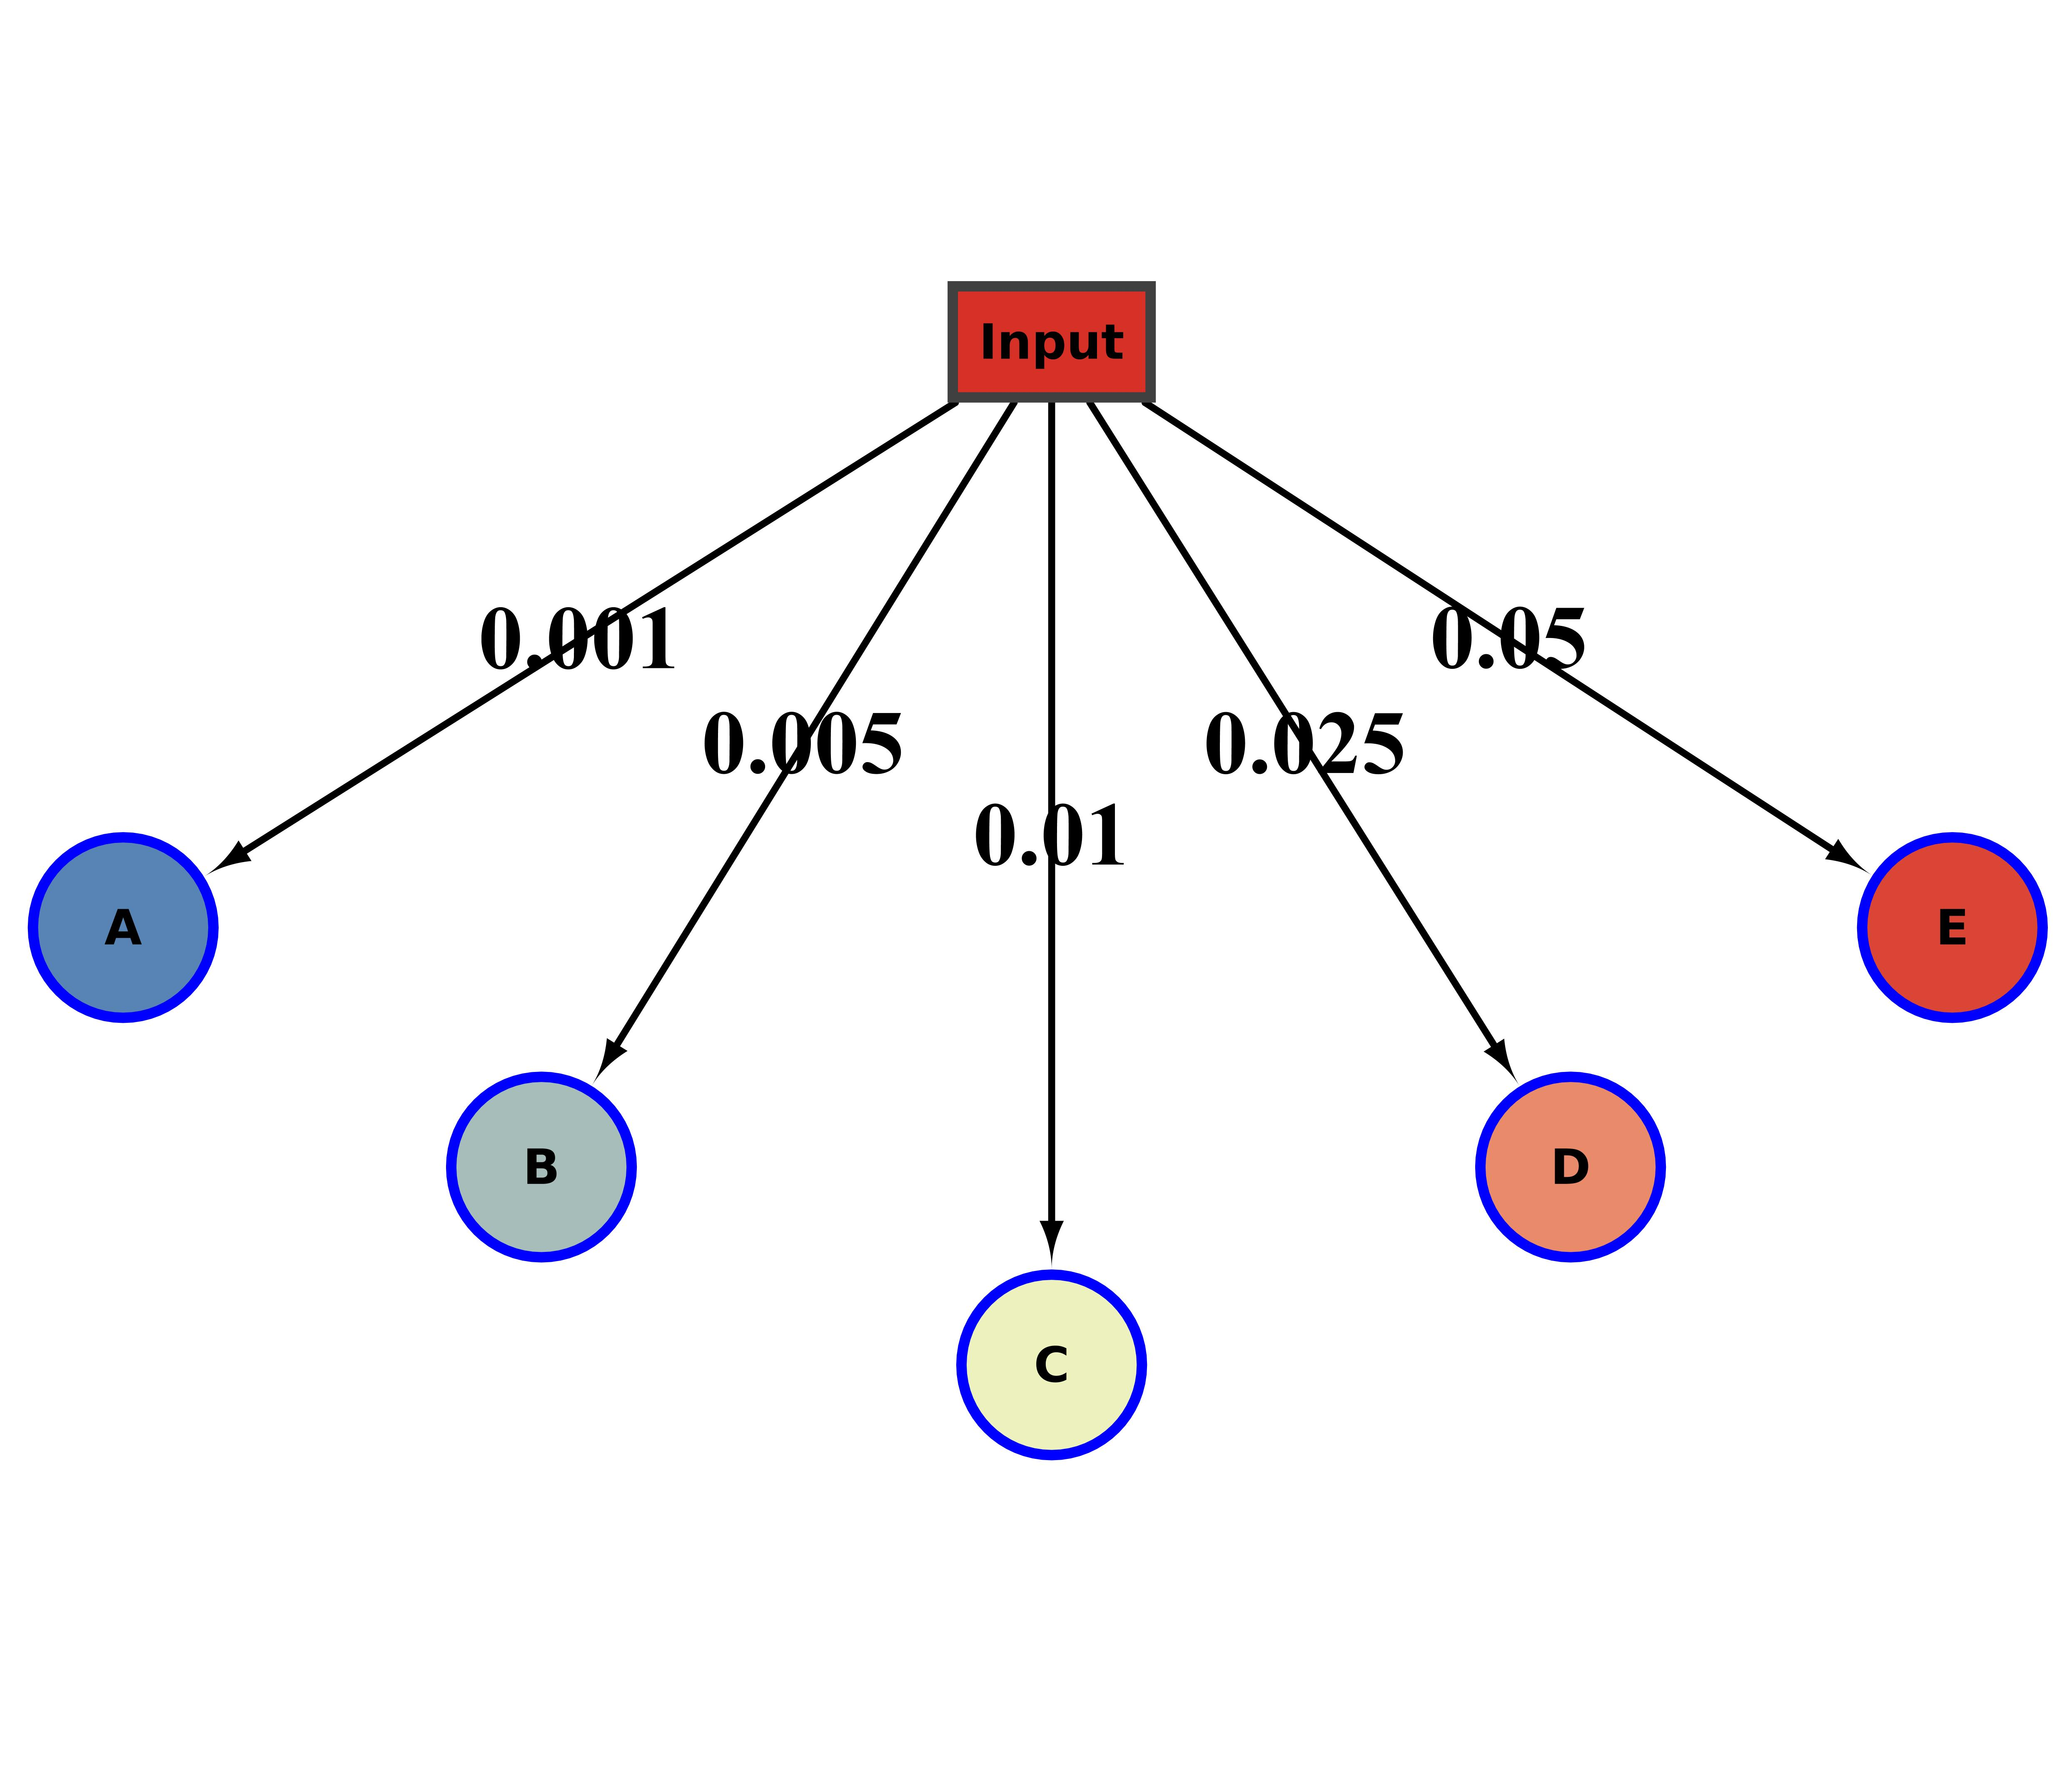
\includegraphics[scale=\graphScale]{parameter_network_CB}} &
% \subfloat[\label{fig:animo-settings-k-graph}]{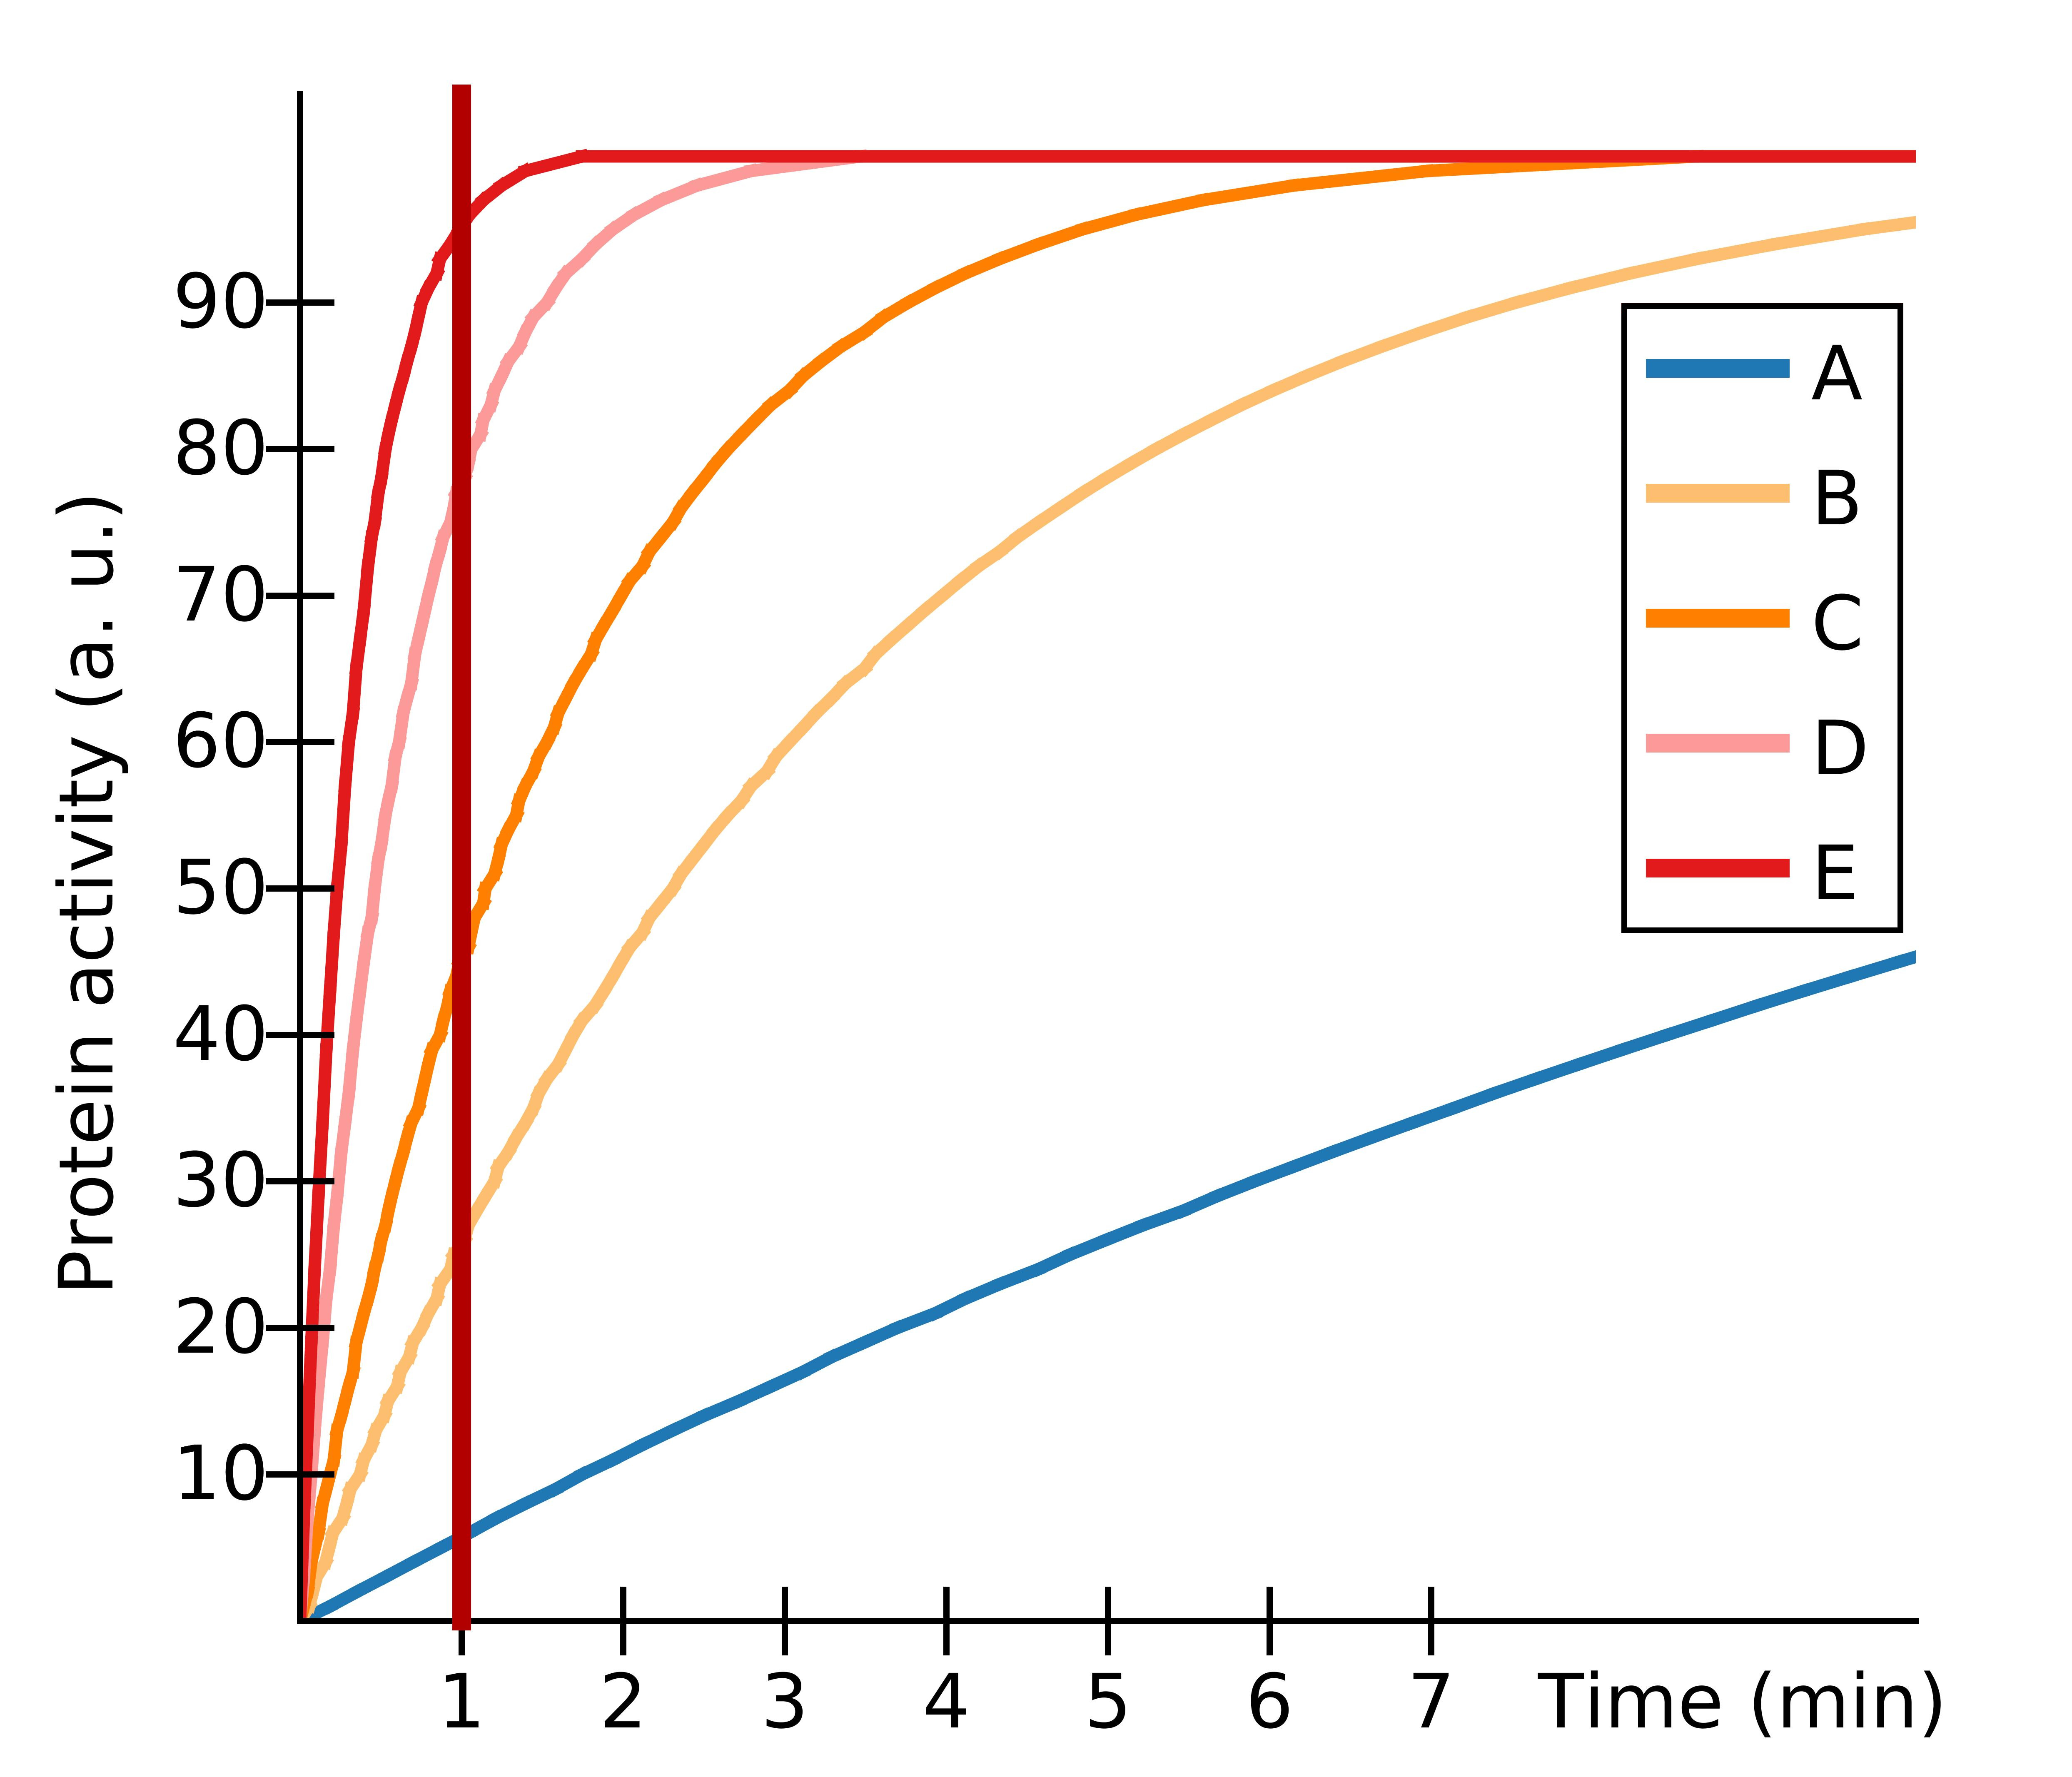
\includegraphics[scale=\graphScale]{parameter_graph}} \\
% \subfloat[\label{fig:animo-settings-direct-network}]{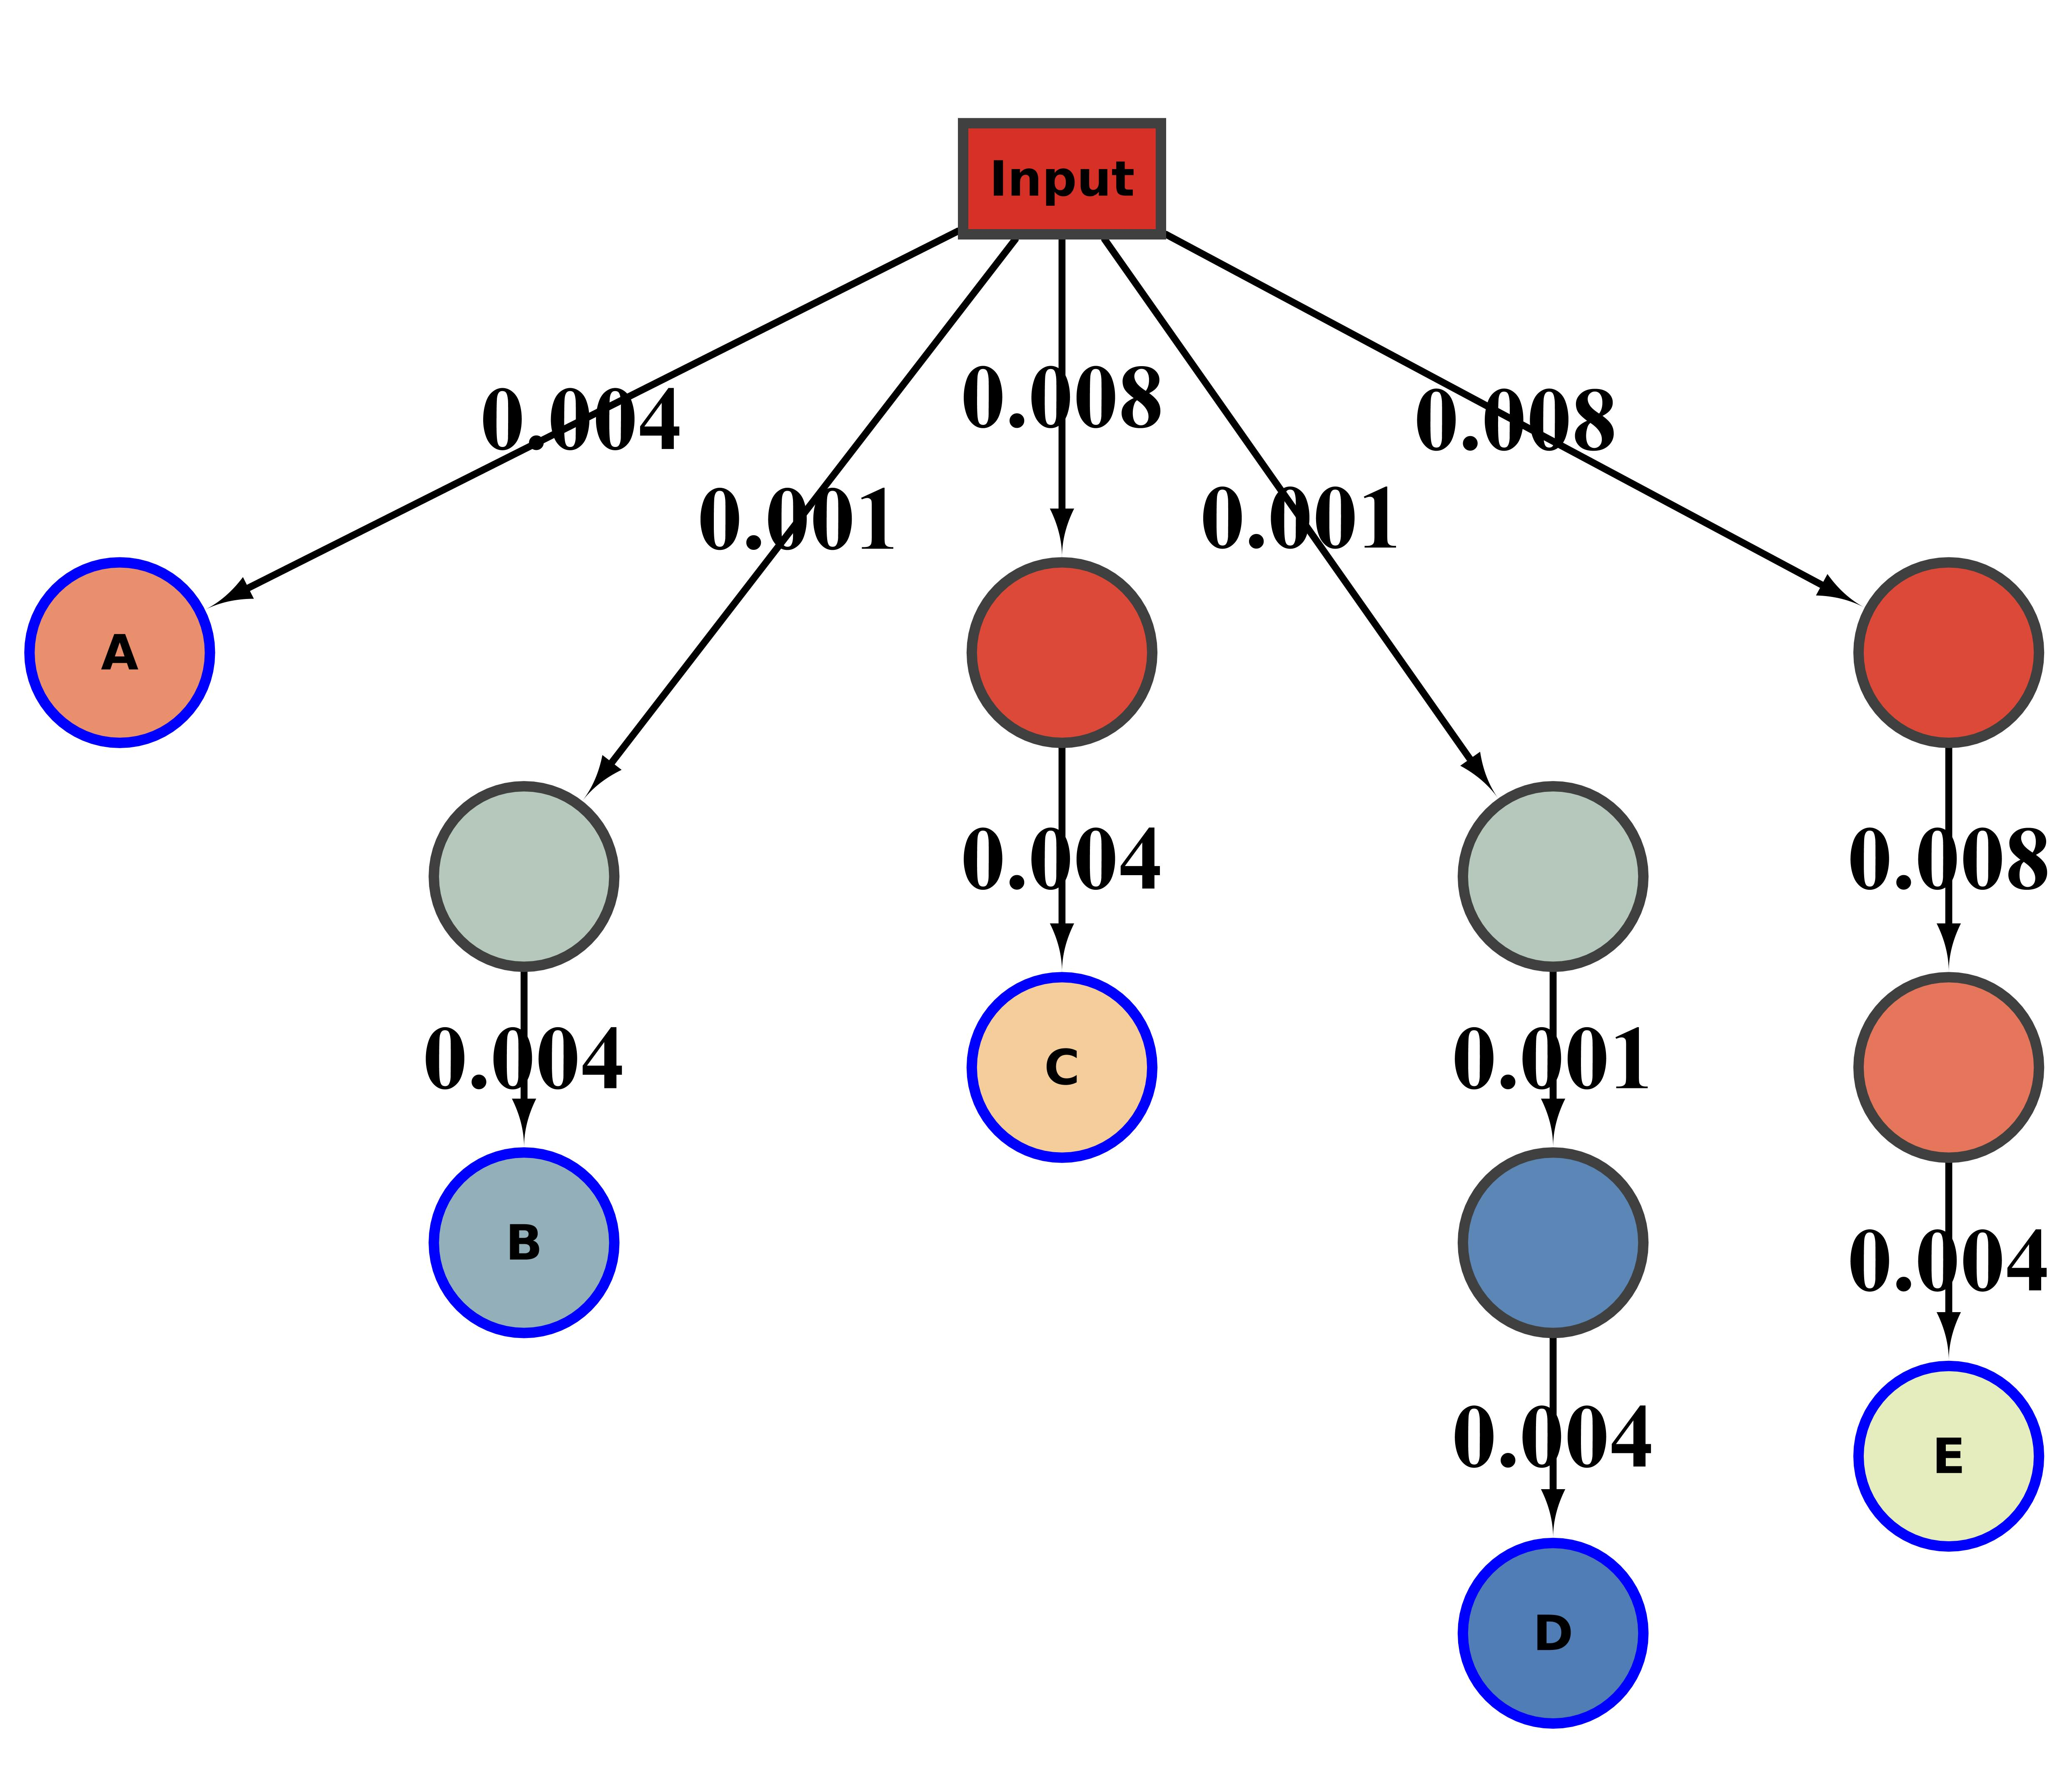
\includegraphics[scale=\graphScale]{direct_indirect_network_CB}} & 
% \subfloat[\label{fig:animo-settings-direct-graph}]{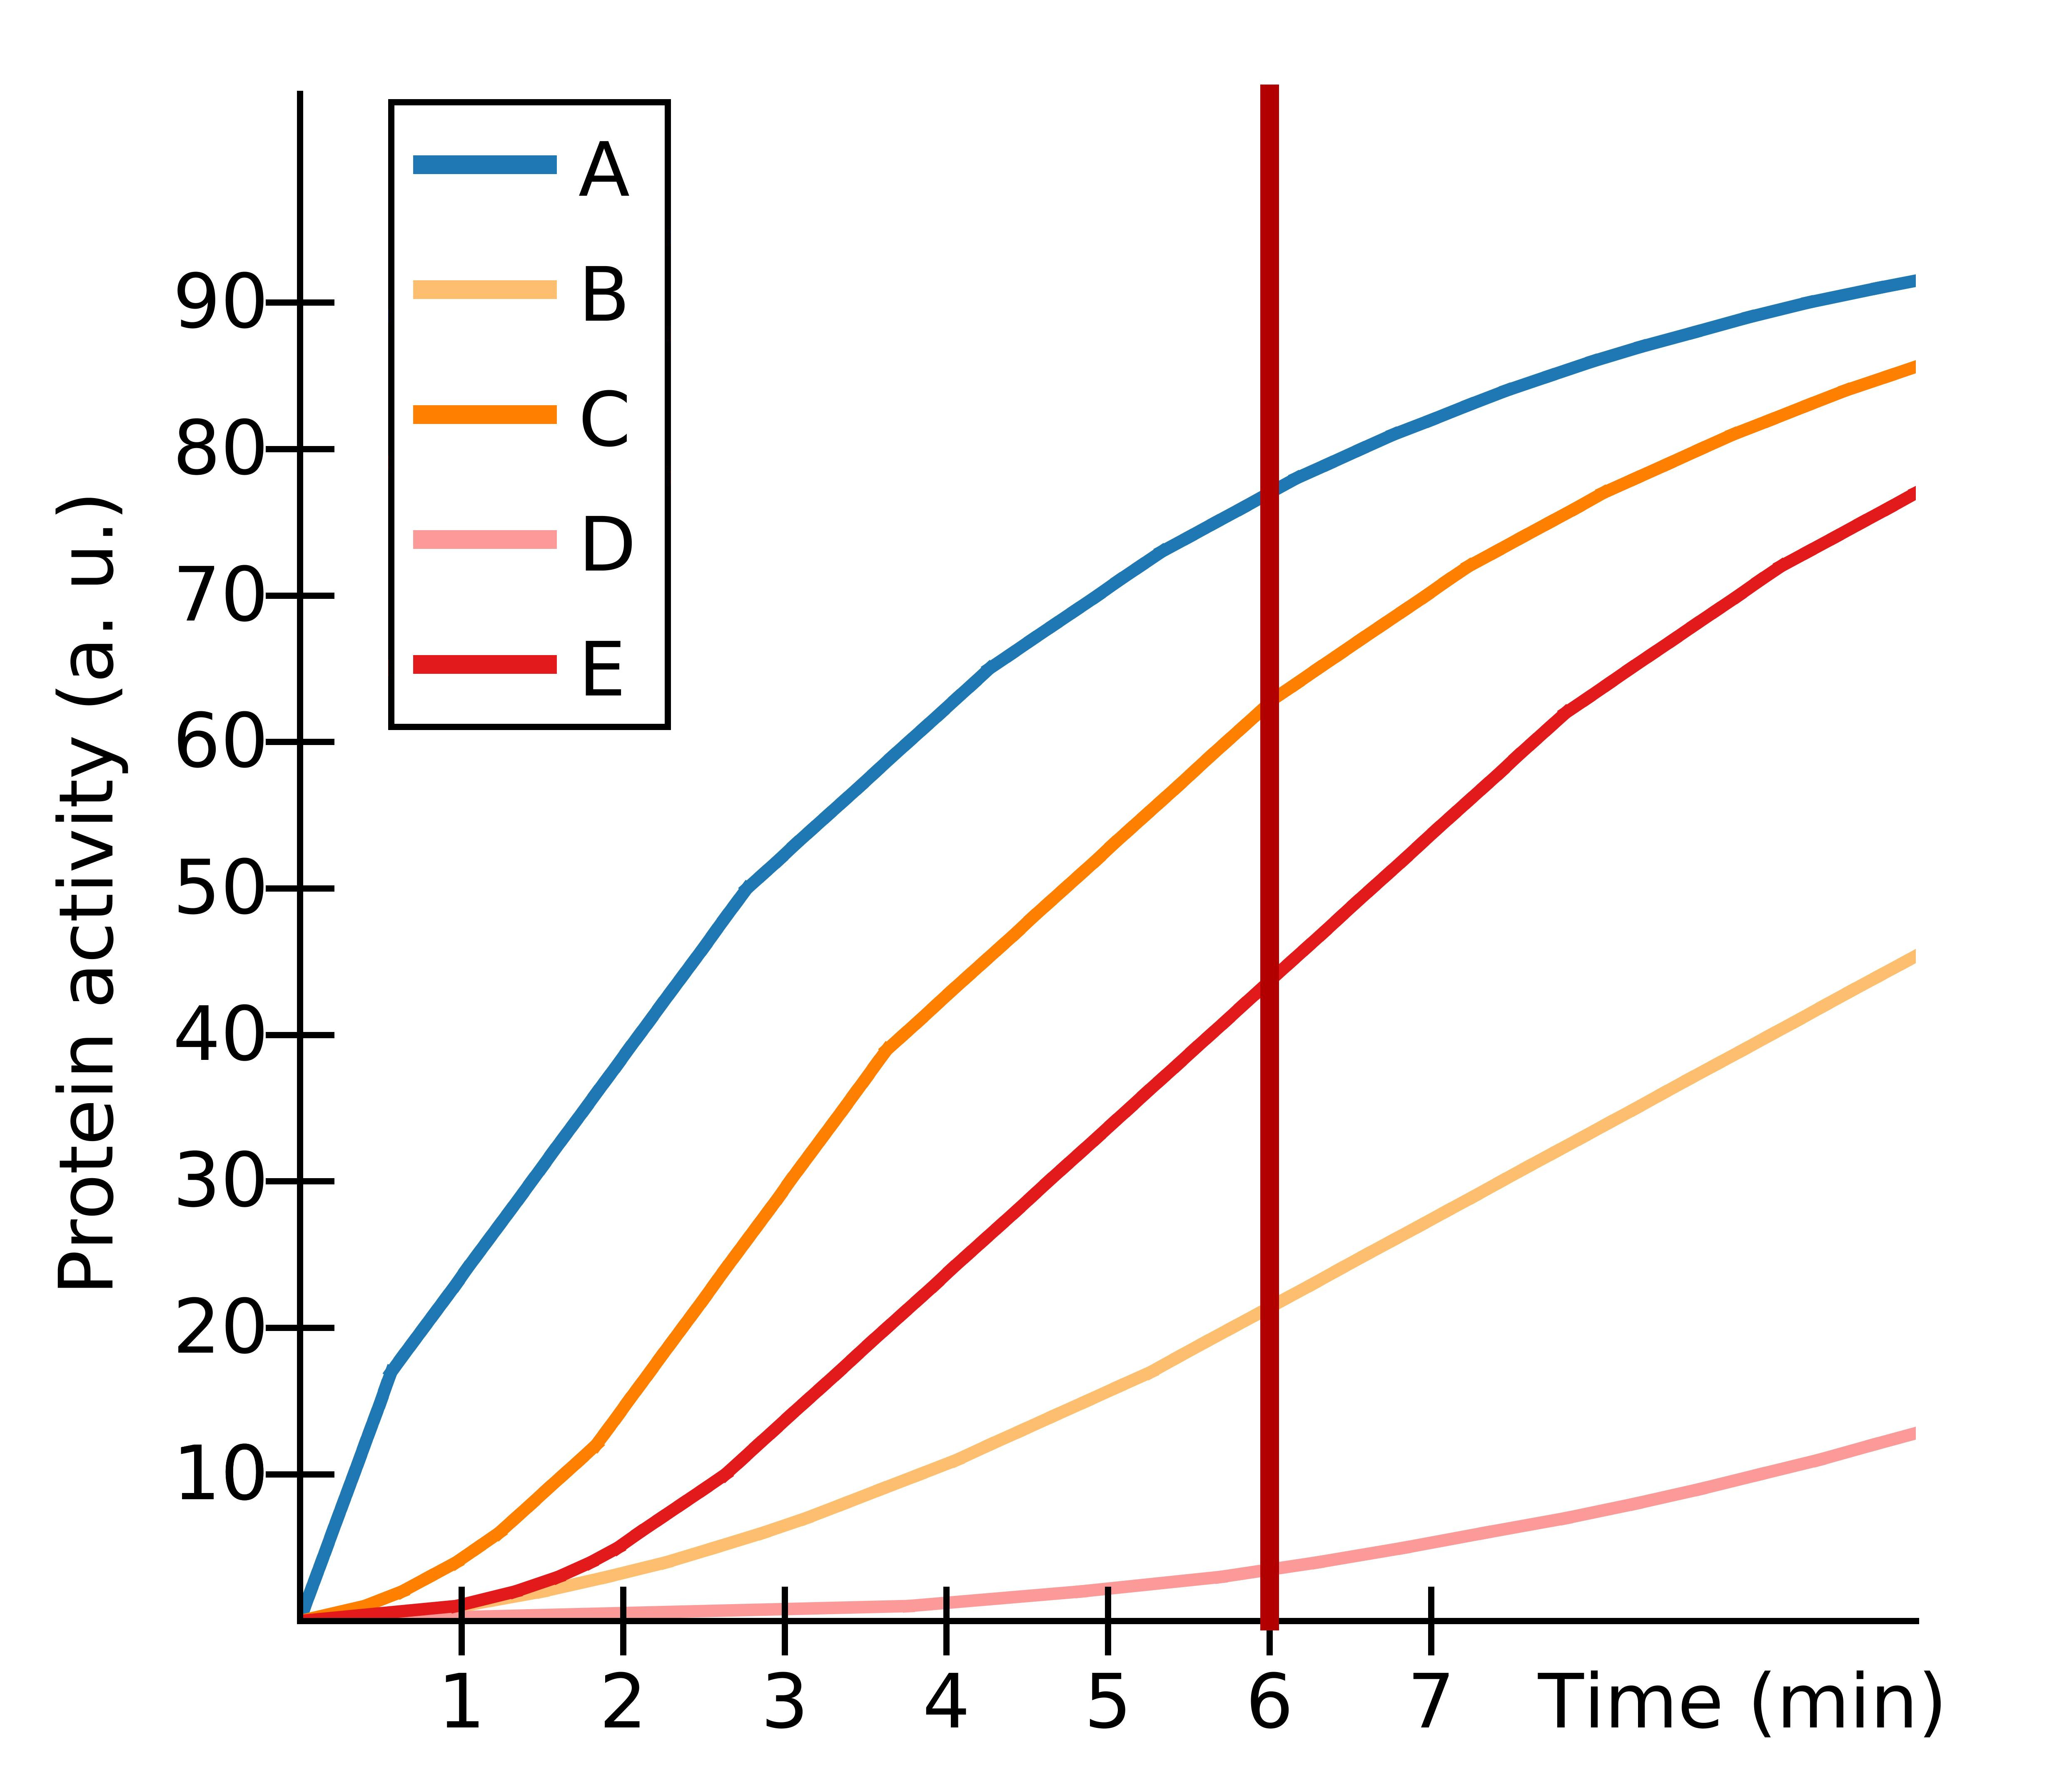
\includegraphics[scale=\graphScale]{direct_indirect_graph}} & 
% \subfloat[\label{fig:animo-settings-feedback-network}]{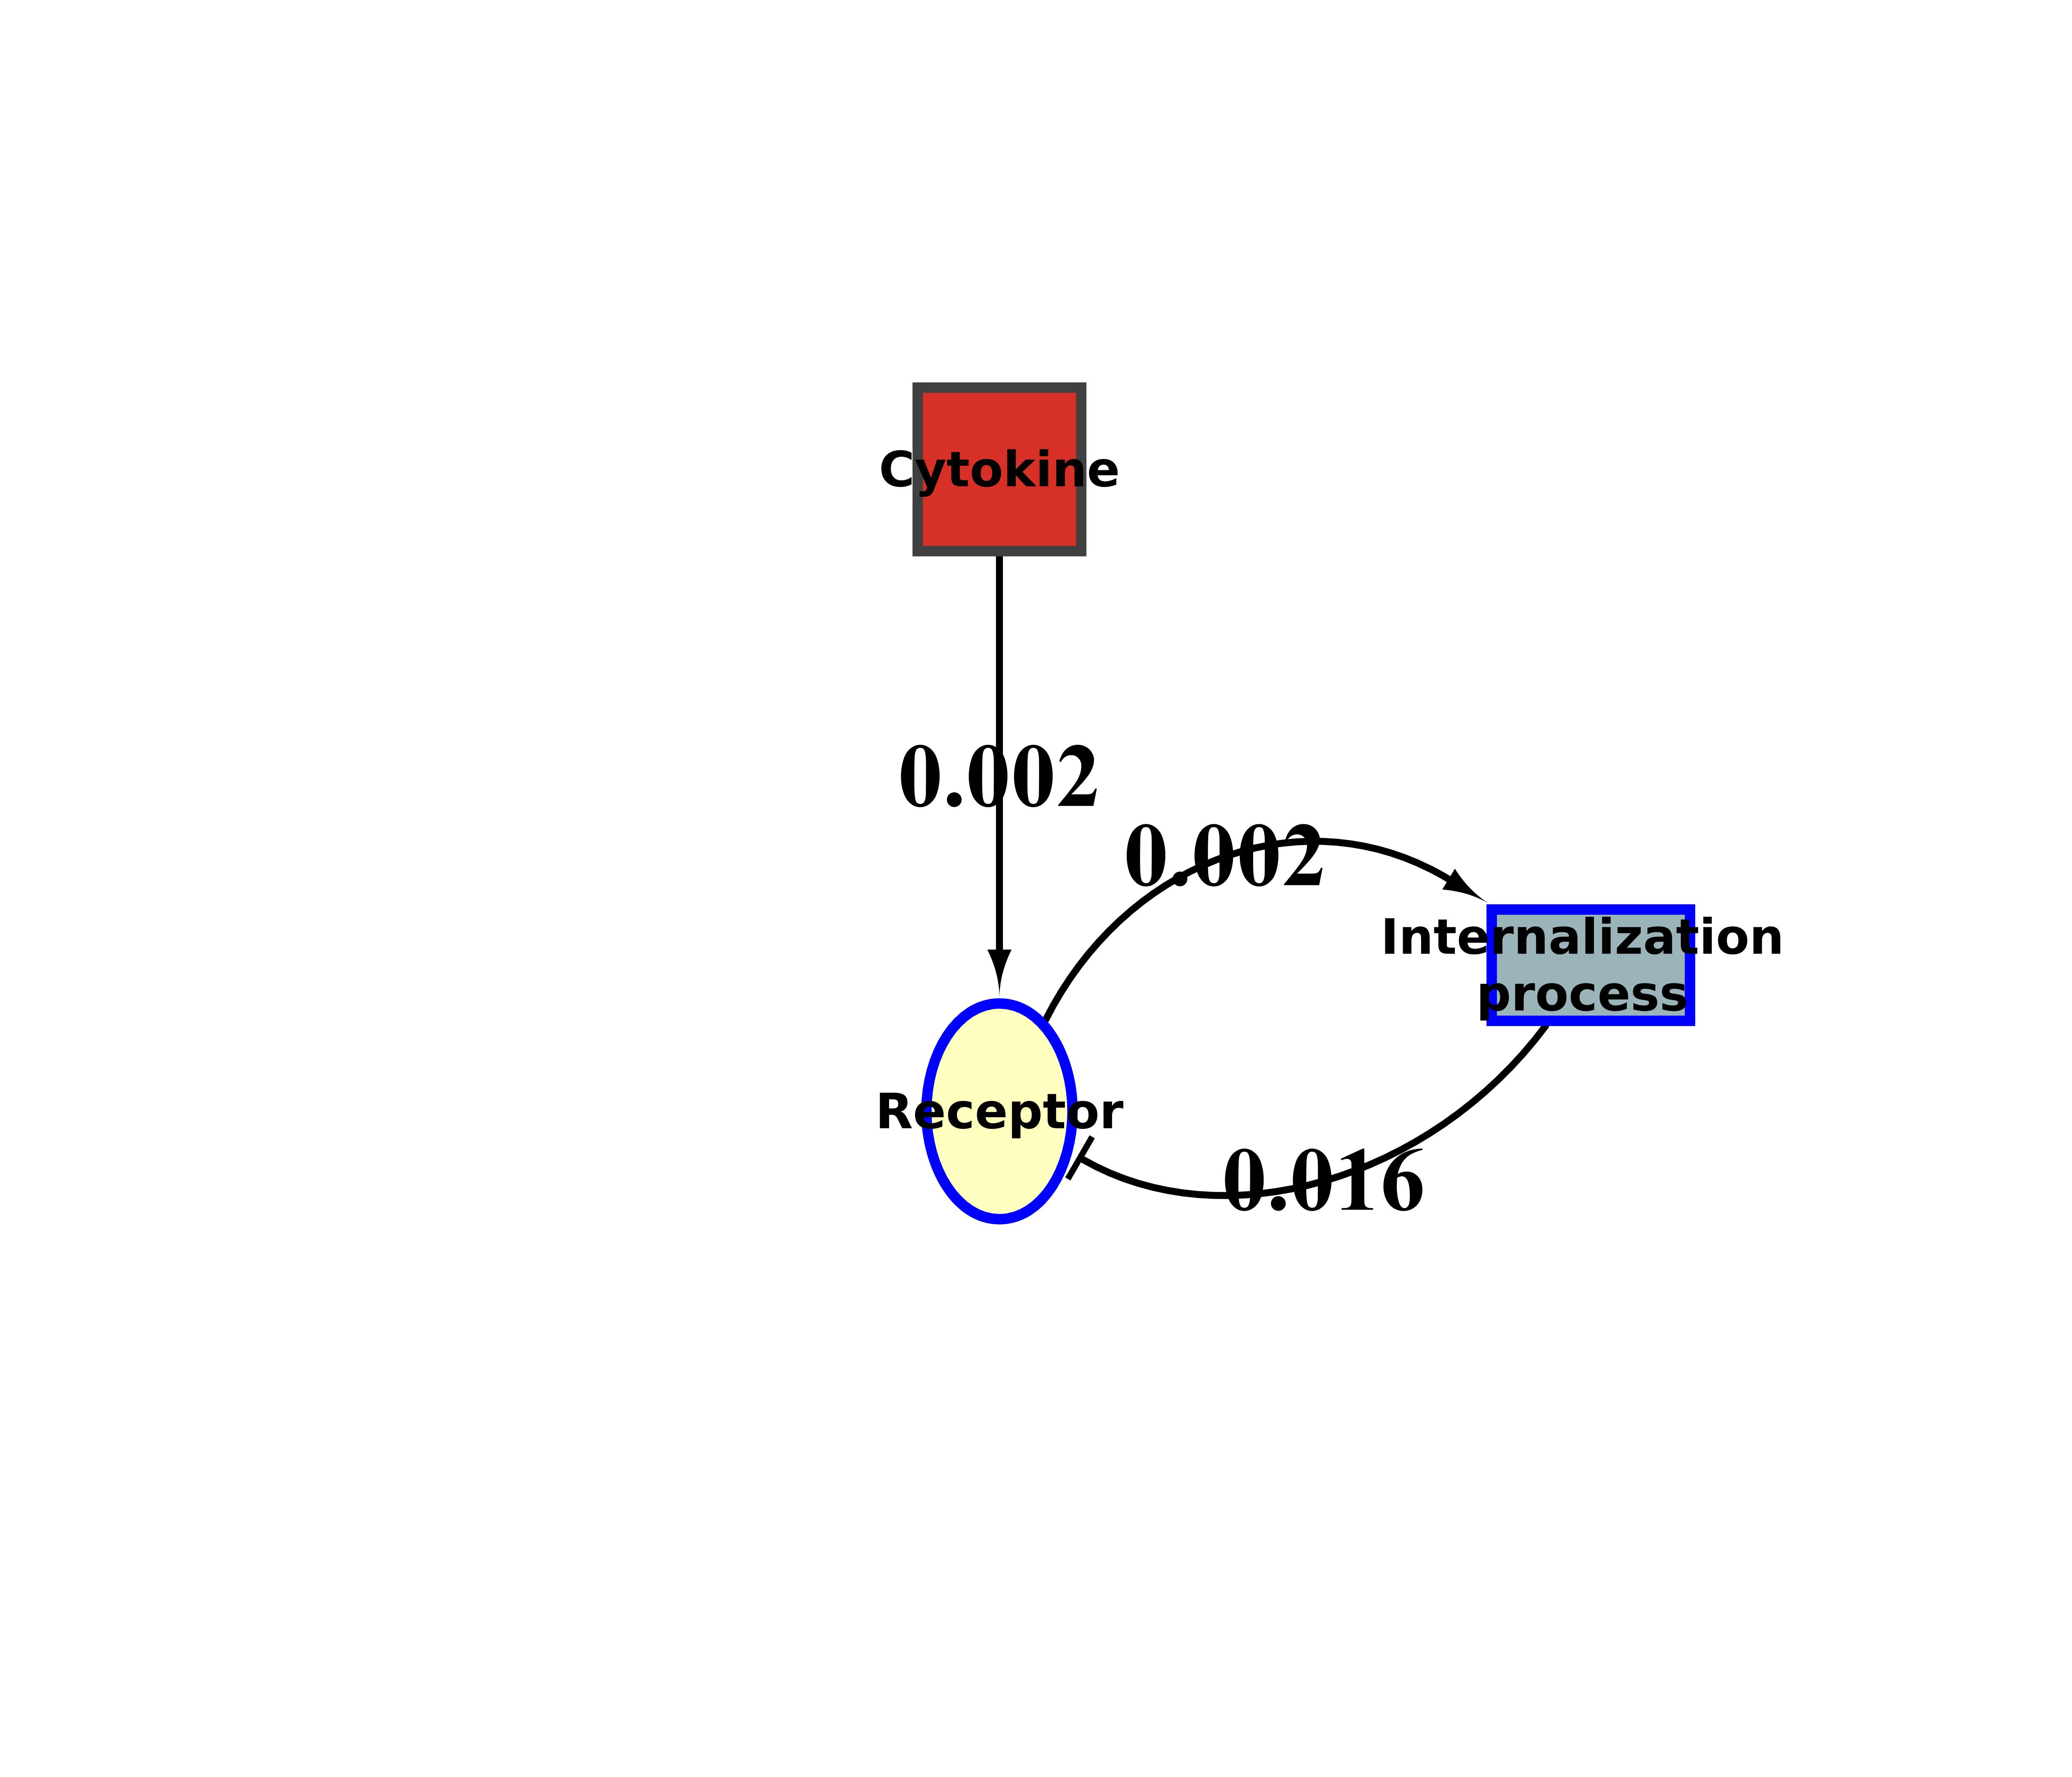
\includegraphics[scale=\graphScale]{feedback_network_CB}} & 
% \subfloat[\label{fig:animo-settings-feedback-graph}]{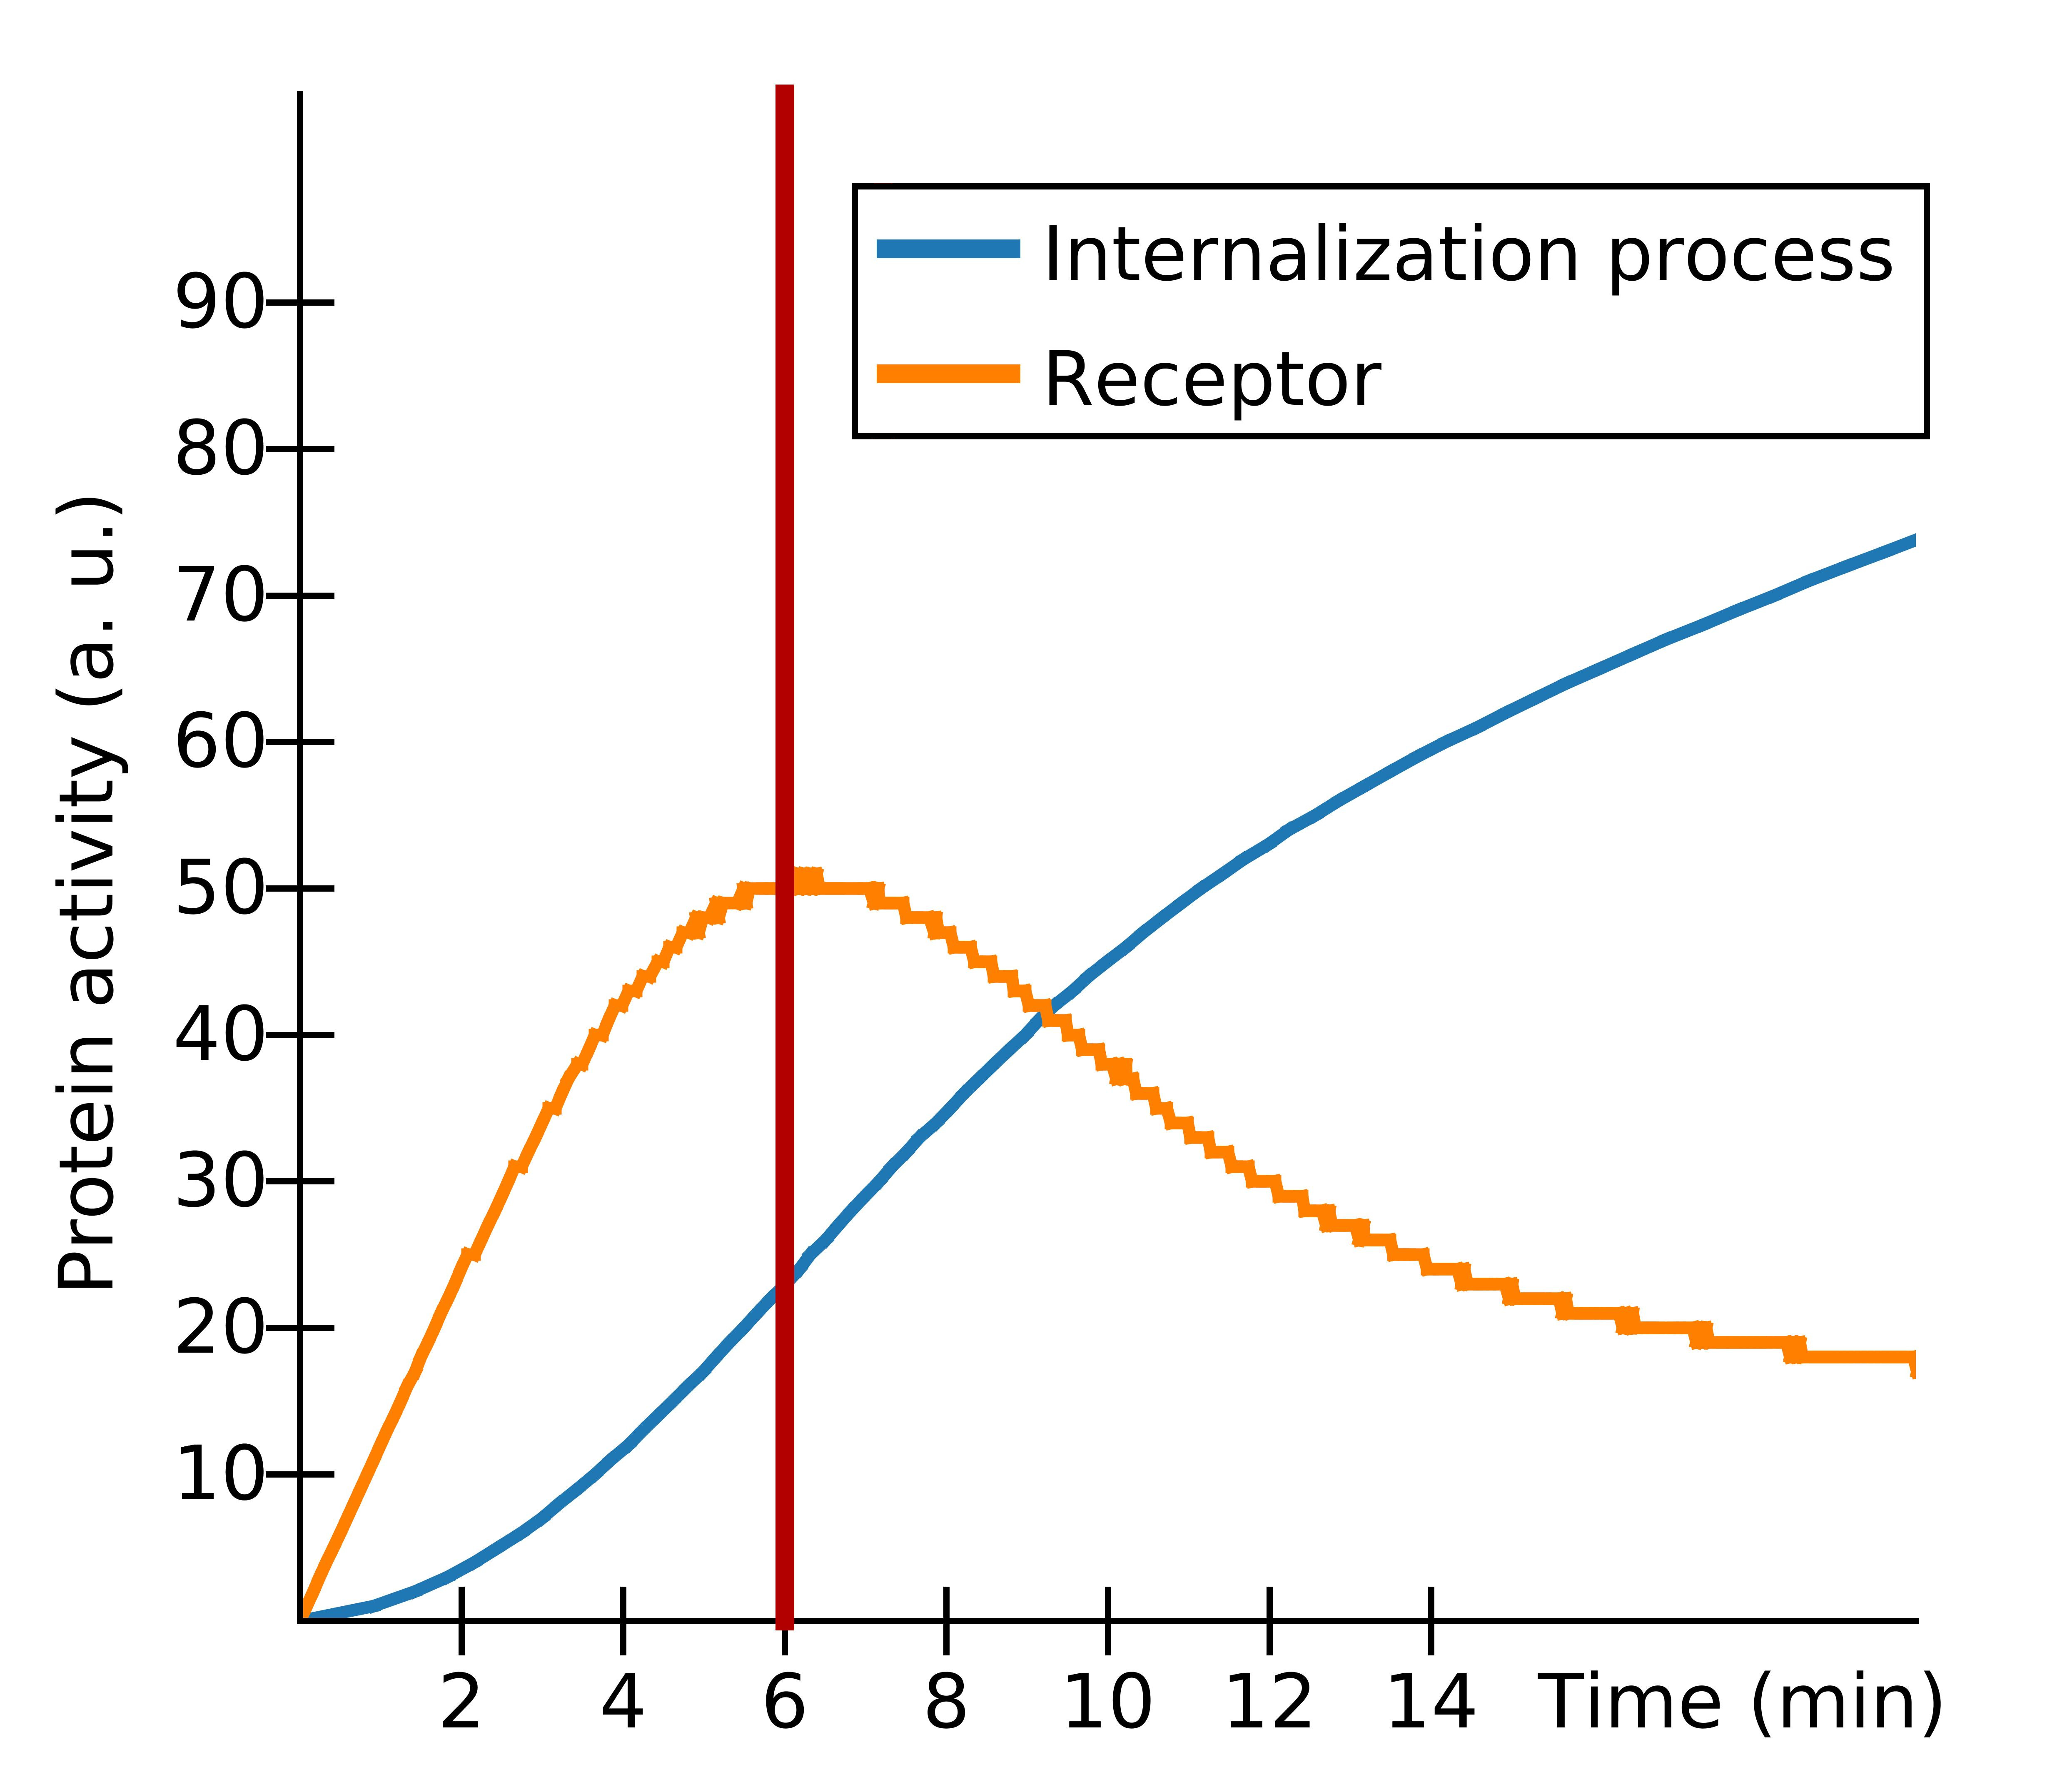
\includegraphics[scale=\graphScale]{feedback_graph}}
% \end{tabular}
% \caption{Example interaction settings for an ANIMO model. Each graph represents the time evolution
% of the network on its left. The vertical red lines in the graphs represent the point in time on which
% the coloration of the nodes in the corresponding network is based.\\
% {\bf ({\protect\subref*{fig:animo-settings-scenario-network}})} The two basic scenarios. Scenario 1
% makes the speed of the interaction depend only on the activity level of the upstream node {\sf Input}. In this case the
% upstream node is constantly active, so the activity of {\sf A} increases linearly with time. Scenario 2
% depends on the activity level of the {\sf Input} node, and on the \emph{inactivity} of {\sf B}. This
% makes the rate of activation of {\sf B} decrease proportionally to the current activity level of {\sf B}:
% the more {\sf B} is active, the slower the activation process will occur.\\
% {\bf ({\protect\subref*{fig:animo-settings-k-network}})} Choosing a value for the scaling factor $k$. While all interactions here
% are based on scenario 2, the value of their parameter $k$ (written on the edges) determines the speed at which the downstream node
% is activated: a larger value of $k$ means a faster reaction.\\
% {\bf ({\protect\subref*{fig:animo-settings-direct-network}})} Relation between network topology and delays. In order to delay the activation process
% ensuing an external signal (node {\sf Input}), we can reduce the reaction speed by changing $k$ or
% adding an intermediate node. Introducing a slowly activated ($k = 0.001$) node between {\sf Input} and {\sf B} is enough to
% activate {\sf B} at a much slower rate than {\sf A}, even if the value of $k$ for the last step is left unchanged at $k = 0.004$.
% Increasing the parameter of the newly introduced reaction lets us fine tune
% the speed of the response, making the activation of {\sf C} faster than {\sf B}, but still slower than {\sf A}. We repeat the process
% of introducing a delay with nodes {\sf D} and {\sf E}: an additional intermediate node further reduces the response time.\\
% {\bf ({\protect\subref*{fig:animo-settings-feedback-network}})} Peak dynamics are often observed in experimental data.
% In order to have the activity level of a node increase and successively decrease, the simplest way is to model it with a feed-back loop.
% In the example, we model the internalization of a receptor following its activation. Note that the interaction {\sf Internalization
% process} $\dashv$ {\sf Receptor} is an inhibition: being based on scenario 2, it will reduce the activity of the {\sf Receptor} node with a rate proportional
% to the current activity of both involved nodes. Scenario 1 dynamics are sufficient to model the two activating reactions {\sf Cytokine} $\rightarrow$ {\sf Receptor}
% and {\sf Receptor} $\rightarrow$ {\sf Internalization Process}. Key to the peak dynamics is the fact that the inactivation of the {\sf Receptor} node
% is much faster (higher $k$ value) than its activation.
% \label{fig:animo-networks}}
% \end{figure*}
